%\documentclass[pra,showpacs,twocolumn]{revtex4}
\documentclass[preprint]{revtex4-2}
%%%%%%%%%%%%%%%%%%%%%%%%%%%%%%%%%%%%%%%%%%%%%%%%%%%%%%%%%%%%%%%%%%%%%%%%
\usepackage{amssymb}
\usepackage{amsmath}
\usepackage{graphicx}
\usepackage{multirow}
\usepackage{gensymb}
\usepackage{float}
\usepackage{MnSymbol}
\usepackage{gensymb}



\begin{document}

\title{Ionization of biological molecules by multicharged ions by using 
the stoichiometric model}

\author{author}
\address{Instituto de Astronom\'{\i}a y F\'{\i}sica del Espacio 
(CONICET-UBA).
Casilla de correo 67, sucursal 28 (C1428EGA) Buenos Aires, Argentina.}
\author{author}
\affiliation{Instituto de Astronom\'{\i}a y F\'{\i}sica del Espacio (CONICET-UBA).
Casilla de correo 67, sucursal 28 (C1428EGA) Buenos Aires, Argentina.}
\affiliation{Fac. de Ciencias Exactas y Naturales, Universidad de Buenos Aires}

\date{\today}% It is always \today, today,

\begin{abstract}
In this work we investigate the ionization of molecules of biological 
interest by impact of multicharged ions in the intermediate to high 
energy range. We performed full non--perturbative distorted--wave 
calculations (CDW) for thirty six collisional systems, six charged projeciles 
(antiprotons, H, He, B, C and O) and by six atomic targets H, C, N, O, 
F and S. These atoms are the constituents of most of the DNA and 
biological molecules. By considering the stoichiometric composition of 
the different molecules we approximate the ionization cross sections 
as linear combination of the atomic ones.  We show that this simple 
stoichiometric model (SSM) gives reasonable good results for complex 
molecules. We focused on seventeen molecules including the DNA 
(adenine, cytosine, guanine, thymine, uracil), DNA backbone, the 
pyrimidines, tetrahydrofuran (THF), and the C$_n$H$_n$ compounds. The 
full comparison of 
the total ionization cross sections for the different ions normalized 
to the square of the ion charge gives an interesting picture of the
experimental state of art. The energy and angular distributions of the 
emitted electrons are also inspected due to its relation with the 
radiation damage. Our results show that these two parameters are highly 
dependent on the projectile charge state, which cannot be noted in a
first order perturbative calculation. We also analyze the extensively 
used Toburen 
scaling of the total ionization cross sections of molecules with the 
number of weakly bound electrons. We tested this scaling for the seventeen 
different molecules and the six projectiles per each, which allows to 
have an insight on the limitation of this scaling. Instead, based on 
the present CDW results for the atoms, we propose a different number 
of electrons per atom. This CDW--based scaling highly improves the 
single curve behaviour for all the targets and ions studied here, in the 
intermediate to high energy region. The new scaling also describes well 
the available experimental data, including small molecules such as H2, 
water, methane and ammonia. For completeness, we performed full 
molecular calculations for the five DNA molecules, and tested a 
corrected stoichiometric formula based on the actual number of 
electrons around each molecular center. The difference of these more 
realistic ionization cross sections and the SSM ones was less than 
$3\%$, being an indication of the reliability and robustness of the 
SSM to deal with this type of molecules. Based on the extensive 
ion-target systems included in the present study, and the results 
obtained, the possibilities of the SSM and the new scaling are of 
great impact.
\end{abstract}

%\keywords{Suggested keywords}

\maketitle

%\tableofcontents
%\pacs{79.20.Rf, 68.49.Bc, 34.20.Cf,34.50.-s,34.35.+a}

\section{Introduction}

The damage caused by the impact of multicharged heavy projectiles on 
biological targets has become a field of interest due to its recent 
implementation in ion--beam cancer therapy. The effectiveness of the 
radiation depends on the choice of the ions. In particular, theoretical 
and experimental studies with different projectiles have concluded that 
charged carbon ions could be the most suitable ions to be used. 
Nonetheless, the study of such systems represents a challenge from the 
theoretical point of view. 

The ionization of biological molecules by multicharged ions constitutes 
the primary damage mechanism. The most widely used method to predict
such processes is the first Born approximation. At high energies, this 
perturbative method warrants the $Z^{2}$ laws, where $Z$ is the 
projectile charge. However, the damage is concentrated in the 
vicinities of the Bragg peak --at energies of hundreds of keV/amu--, 
precisely where the Born approximation starts to fail. 
Another theoretical issue arises due to the targets themselves; we are 
dealing with complex molecules, and the description of such targets 
represents a hard task for {\it ab initio} calculations. The objective 
of this article is to deal with these two aspects; first, we perform 
more appropriate calculations on the primary damage mechanism, which can 
replace the Born results. Second, we inspect and test a stoichiometric 
model to describe the ionization of molecular targets.

To overcome the first perturbative approximation limitations, and since 
the projectiles are multicharged ions, we resort to the Continuum 
Distorted Wave--Eikonal Initial State (CDW), which includes higher 
perturbative corrections. We start from the premise that the ionization 
process is the mechanism that deposits the most significant amount of 
primary energy. Moreover, it is well known that the residual electrons 
from the ionization become a source of significant local biological 
damage. The secondary electrons are included in Monte Carlo simulations, 
and hence their behavior must be investigated. 
In Section~\ref{subsec:meanener} and \ref{subsec:meanang}, we calculate
the mean energy and angular distributions of the ejected electrons. 
Surprisingly, we found a substantial dependence of the charged 
projectile, which is unexpected in the first Born approximation. 
We deal with the molecular structure complexity of the target by 
implementing the simplest stoichiometric model (SSM): the molecules are 
assumed to be composed of isolated independent atoms, and the total 
cross--section by a linear combination of weighted atomic calculations.

By implementing the CDW and the SSM, we calculate ionization 
cross--section of several molecules of interest (see 
Table~\ref{tab:families}) by the impact of antiprotons, H$^{+}$, 
He$^{+2}$, Be$^{+4}$, C$^{+6}$, and O$^{+8}$. 
In Section~3, we show our results for different DNA and RNA molecules, 
such as adenine, cytosine, guanine, thymine, uracil, tetrahydrofuran~(THF), 
pyrimidine, and also DNA backbone. In Section~\ref{subsec:scaling}, we
test the Toburen scaling rule~\cite{toburen1975,toburen1976}, which 
states that the ratio between the ionization cross--section and the 
number of weakly bound electrons can be arranged in a narrow universal 
band in terms of the projectile velocity. We applied this rule to 
several hydrocarbons and nucleobases and noted that the width of the 
resulting universal band could be significantly reduced if we redefine 
the effective number of active electrons in the collision. The new 
scaling is then tested by comparison with experimental data.

Although the multicharged projectiles are dealt with the CDW, the 
stoichiometric model used seems to be very simplistic. The approach
considers each atom as neutral, which is not correct. In Section 3.5, 
we used the molecular electronic structure code 
{\sc gamess}~\cite{gamess} to calculate the excess or defect of 
electron density on the atoms composing the molecules. Then, the SSM is 
modified to account for the departure from the neutrality of the atoms. 
We find that the modified SSM for the DNA molecules does not introduce 
substantial changes in the cross sections.

%%%%%%%%%%%%%%%%%%%%%%%%%%%%%%%%%%%%%%%%%%%%%%%%%%%%%%%%%%%%%%%%%%%%%%%%
\section{Theory: Ionization of Atoms}
%%%%%%%%%%%%%%%%%%%%%%%%%%%%%%%%%%%%%%%%%%%%%%%%%%%%%%%%%%%%%%%%%%%%%%%%

In the present study, we consider six atoms, $\alpha=$ H, C, N, O, P, 
and S, and six projectiles, antiprotons $\bar{p}$, H$^{+}$, He$^{+2}$, 
Be$^{+4}$, C$^{+6}$, and O$^{+8}$. 
Most of the organic molecules are composed of these atoms. Some 
particular molecules also include halogen atoms such as fluor and 
bromine; ionization cross sections of these elements have been 
previously published~\cite{miraglia2008}.

The total ionization cross sections of these atoms were calculated using 
the CDW~\cite{miraglia2008,fainstein1988,miraglia2009}. The initial bound and final continuum radial wave 
functions were obtained by using the {\sc radialf} code, developed by 
Salvat and co--workers~\cite{salvat1995}, and a Hartree-Fock potential 
obtained from the Depurated Inversion Method~\cite{mendez2016,mendez2018}. 
We used a few thousand pivot points to solve the Schr\"{o}dinger 
equation, depending on the number of oscillations of the continuum 
state. The radial integration was performed using the cubic spline 
technique. The number of angular momenta considered varied from 8, at 
very low ejected-electron energies, up to 30, for the highest energies 
considered. The same number of azimuth angles were required to obtain 
the four-fold differential cross section. The calculation performed does 
not display prior-post discrepancies at all. Each atomic total cross 
section was calculated using 35 to 100 momentum transfer values, 28 
fixed electron angles, and around 45 electron energies depending on the 
projectile impact energy. In our theoretical treatment, we expand our 
final continuum wave function as usual,
\begin{equation}
\psi_{\overrightarrow{k}}^{-}(\overrightarrow{r})=\sum_{l=0}^{l_{\max
}}\sum_{m=-l}^{l}R_{kl}^{-}(r)Y_{l}^{m}(\widehat{r})Y_{l}^{m^{\ast }}
(\widehat{k})\,.
\label{eq:contwave}
\end{equation}
We are confident with our calculations up to $l_{\max}\sim 30$. Further 
details of the calculation are given in Ref.~\cite{montanari2017}. 
Simultaneously, we will be reporting state to state ionization cross 
sections for the 36 ion--target systems considered in the present 
work~\cite{miraglia2019}. A great numerical effort was paid to obtain 
the present results, and we expect that they will be useful to estimate 
molecule fragmentation.

\begin{figure*}[t!]
\centering
\includegraphics[width=0.75\textwidth]{figuras/Fig_finales/Fig1.eps}
%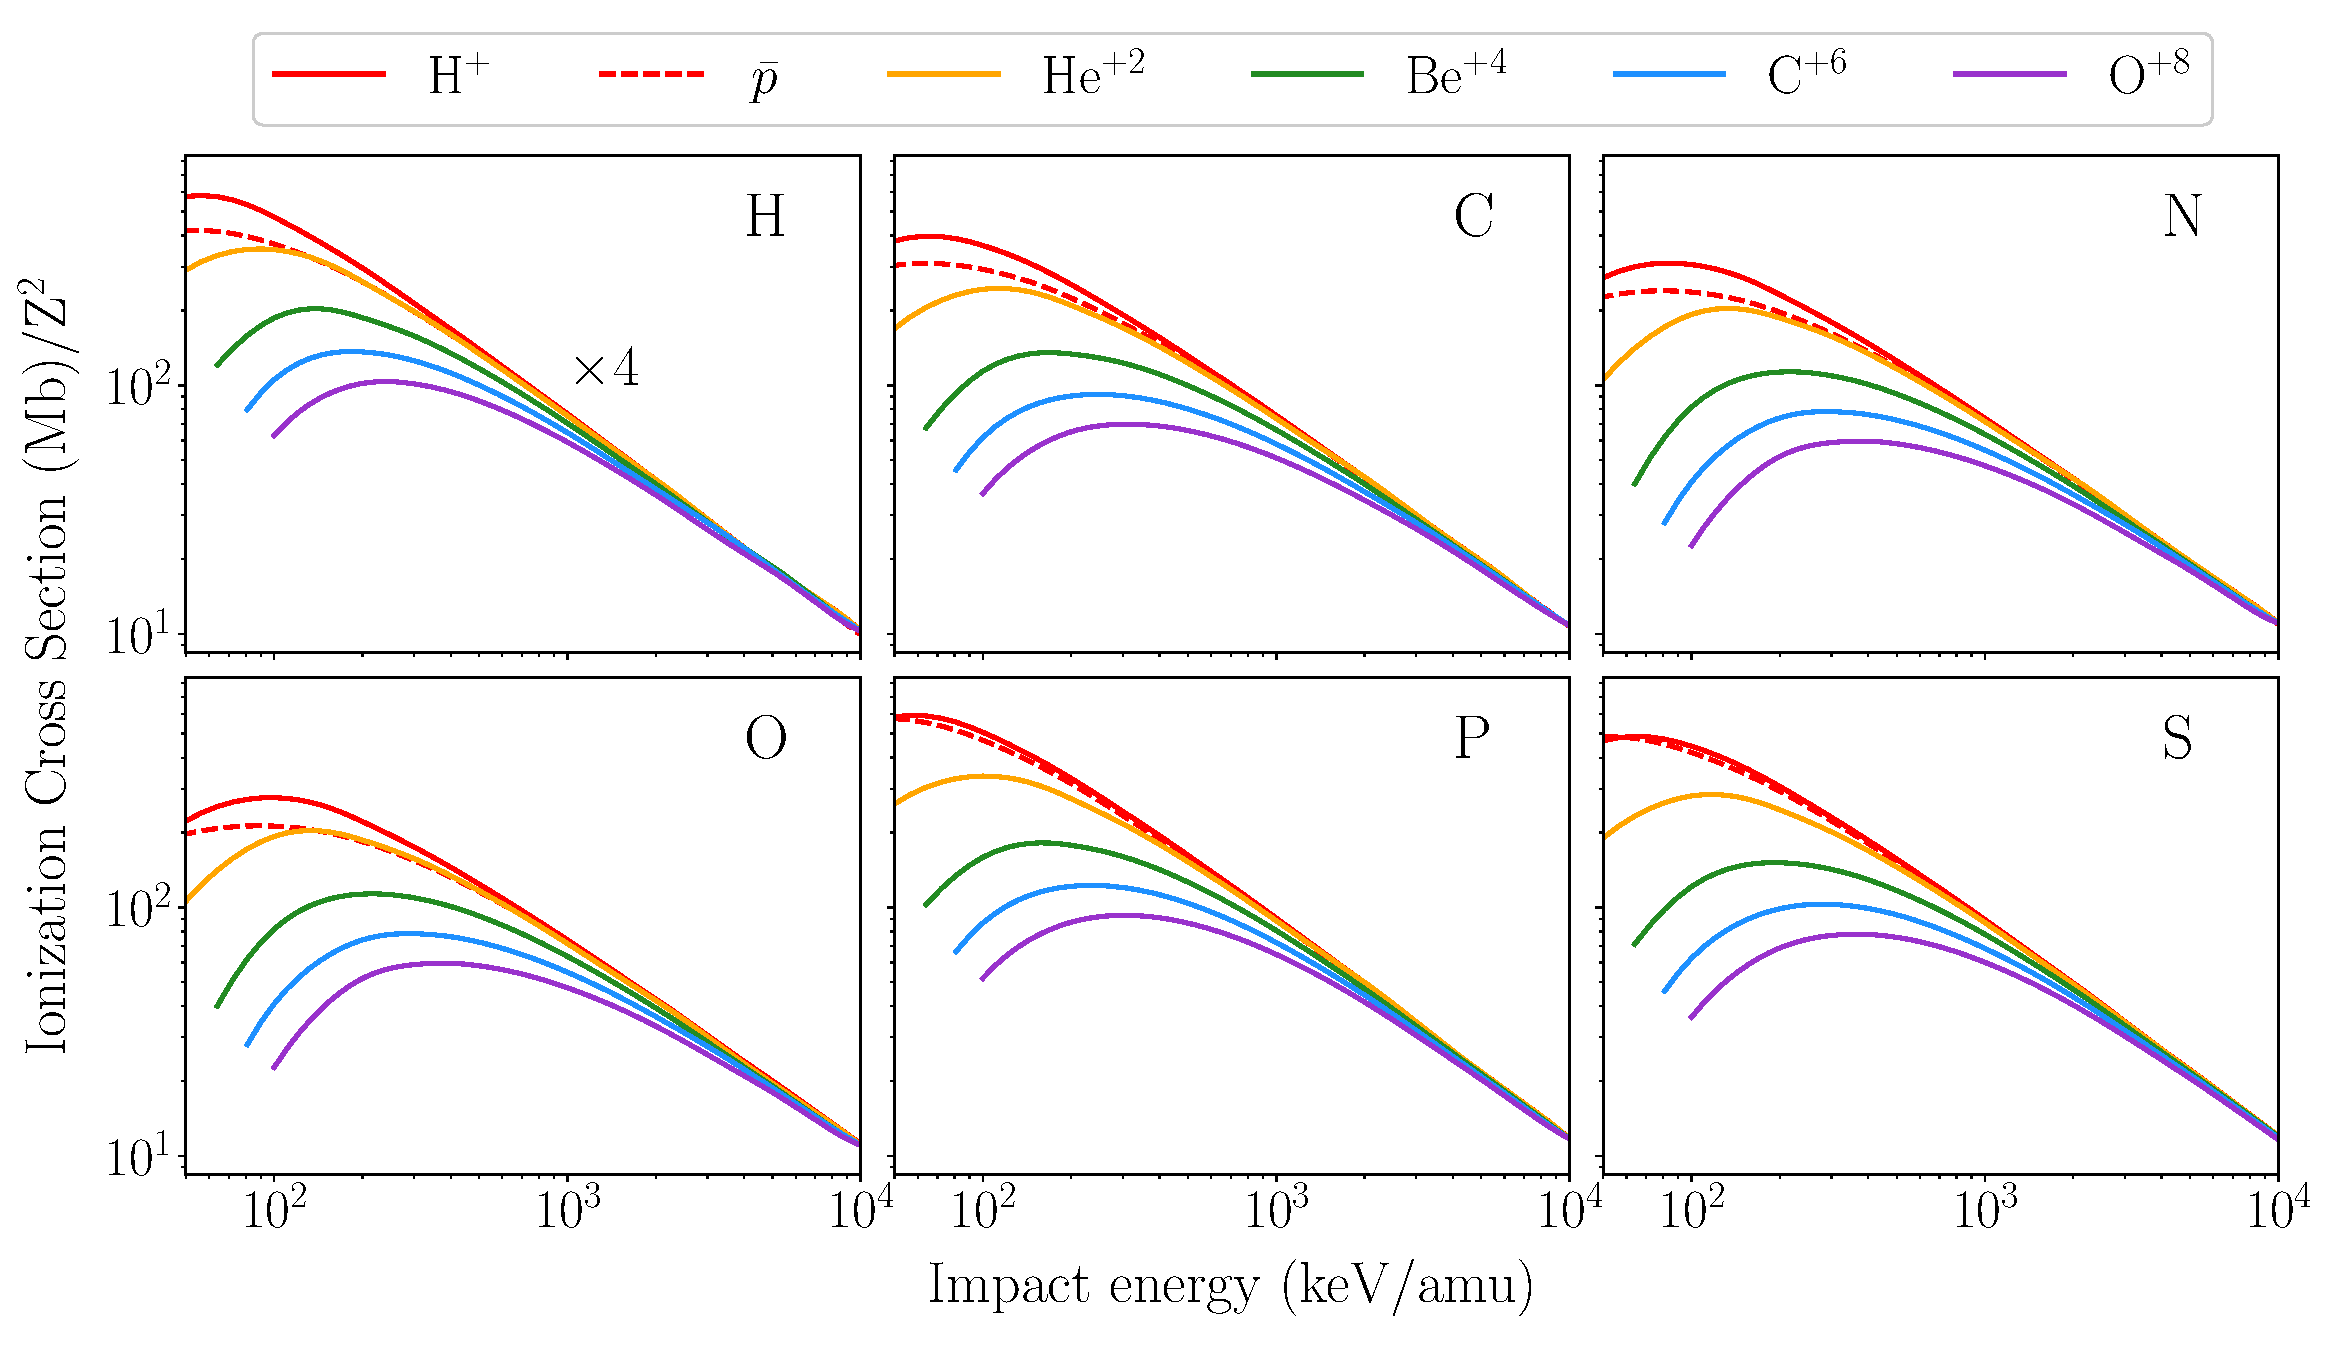
\includegraphics[width=0.9\textwidth]{figuras/atomicscaling.eps}
\caption{Reduced CDW total ionization cross section of six atomic 
targets. The curves are labeled with the charge state corresponding to 
the six multicharged projectiles.}
\label{fig:atomscaling}
\end{figure*} 

We report our total CDW ionization cross sections for the six essential 
elements by the impact of six projectiles in Fig.~\ref{fig:atomscaling}.
To reduce the resulting 36 magnitudes into a single consistent 
figure, we considered the fact that in the first Born approximation
the ionization cross section scales with the square of the projectile 
charge, $Z^{2}$. The values of the impact energies considered 
range between 0.1 to 10 MeV/amu, where the CDW is supposed 
to hold. In fact, for the highest projectile charges the minimum 
impact energy where the CDW is expected to be valid could be 
higher than 100 keV. We also performed similar calculations with the 
first Born approximation, and we corroborated that it provides quite 
reliable results only for energies higher than a couple of MeV/amu. 
We use the same line color to indicate the projectile charge throughout 
all the figures of this work: dashed--red, solid--red, blue, magenta, 
olive and orange for antiprotons, H$^{+}$, He$^{+2}$, Be$^{+4}$, 
C$^{+6}$, and O$^{+8}$, respectively. Notably, there is no complete 
tabulation of ionization of atoms by the impact of multicharged ions. 
We hope that the ones presented in this article will be of help for 
future works.


%%%%%%%%%%%%%%%%%%%%%%%%%%%%%%%%%%%%%%%%%%%%%%%%%%%%%%%%%%%%%%%%%%%%%%%%
\subsection{Emitted electron energies}
\label{subsec:meanener}
%%%%%%%%%%%%%%%%%%%%%%%%%%%%%%%%%%%%%%%%%%%%%%%%%%%%%%%%%%%%%%%%%%%%%%%%

In a given biological medium, direct ionization by ion impact accounts 
for just a fraction of the overall damage. Secondary electrons, as well 
as recoil target ions, also contribute substantially to the total damage. 
We can consider the single differential cross section of the shell 
$nl$ of the atom $\alpha$, $d\sigma_{\alpha nl}/dE$, to be a function 
of the ejected electron energy $E$ as a simple distribution 
function~\cite{surdutovic2018}. Then, we can define the mean value 
$\overline{E}_{\alpha}$ as in Ref.~\cite{abril2015},
\begin{eqnarray}
\overline{E}_{\alpha} &=&\frac{\langle E_{\alpha}\rangle}{\langle
1\rangle}=\frac{1}{\sigma_{\alpha}}\sum\limits_{nl}\int dE\,E
\frac{d\sigma_{\alpha,nl}}{dE}\,,  
\label{40} \\
\langle 1\rangle &=&\sigma_{\alpha}=\sum\limits_{nl}\int dE\,
\frac{d\sigma_{\alpha,nl}}{dE}\,,  
\label{50}
\end{eqnarray}
where $\Sigma_{nl}$ takes into account the sum of the different 
sub--shell contributions of the element $\alpha$.

\begin{figure*}[t!]
\centering
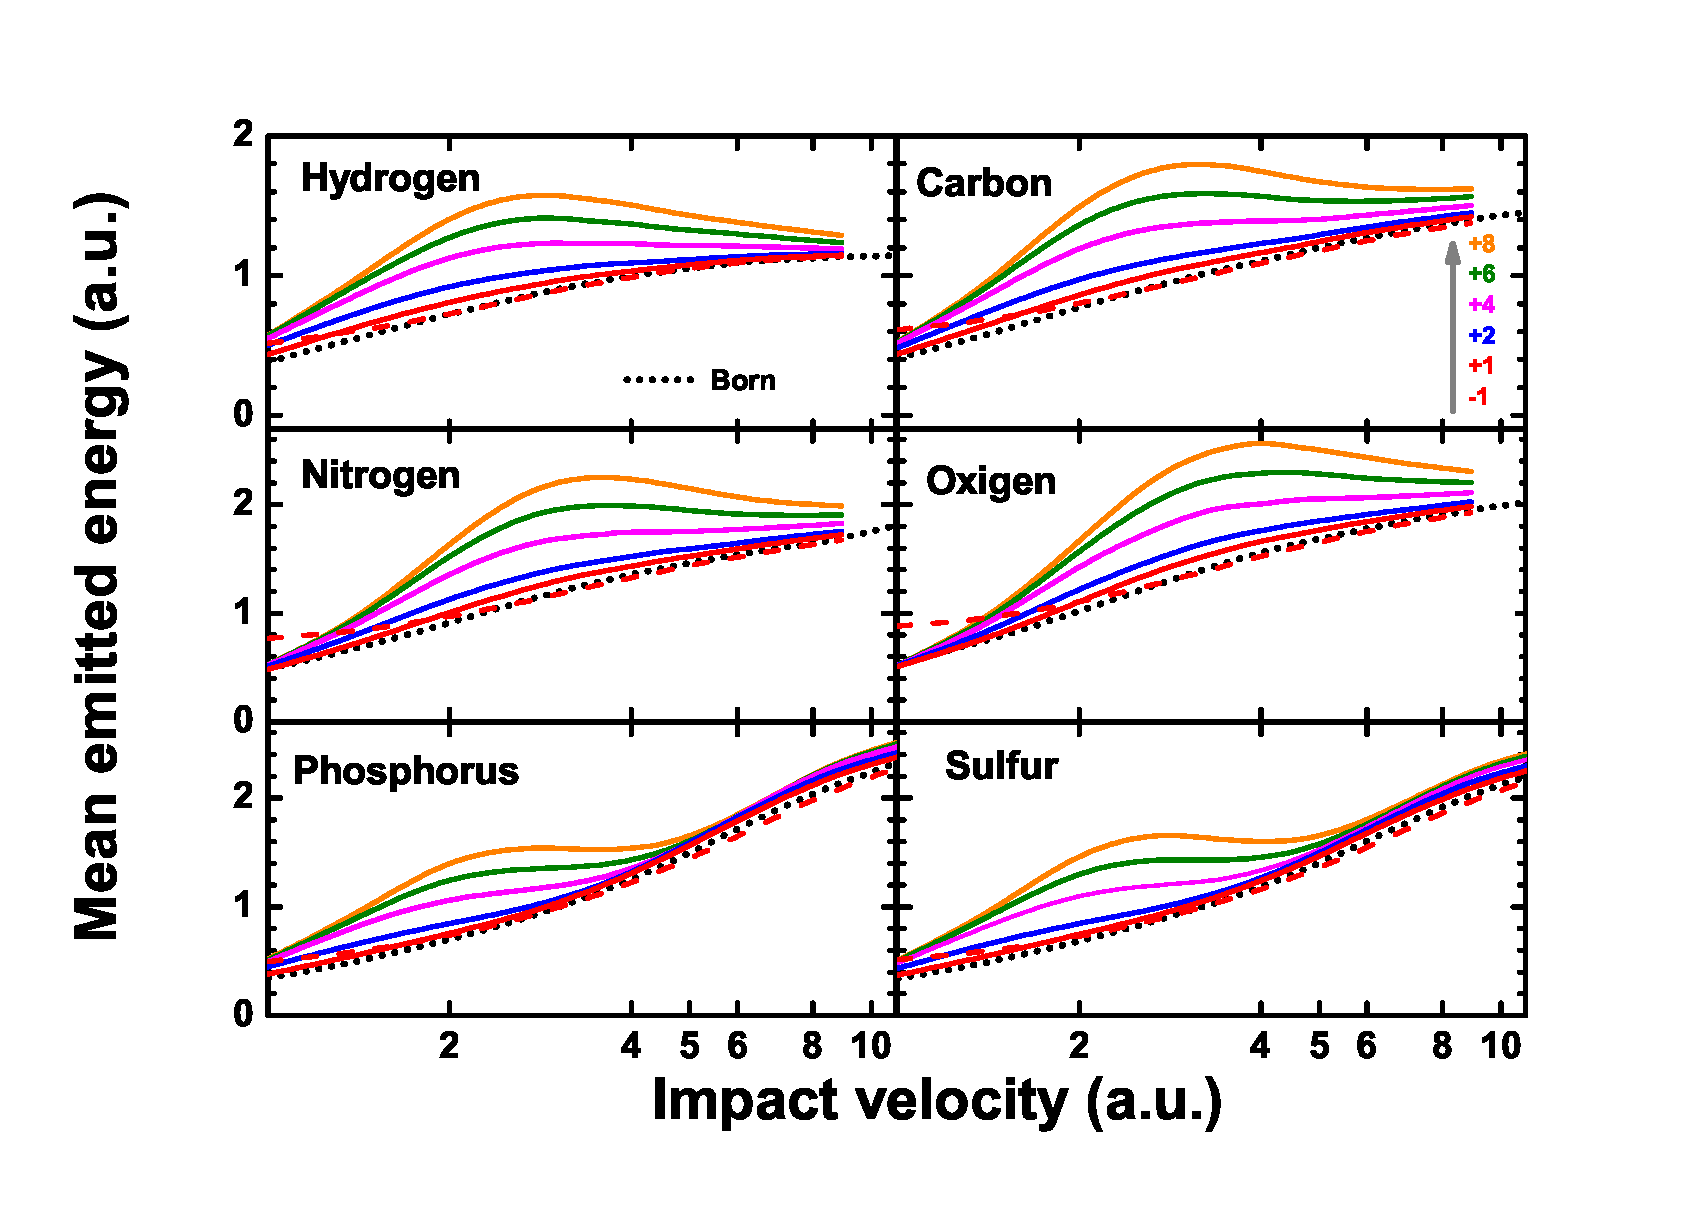
\includegraphics[width=0.75\textwidth]{figuras/Fig_finales/fig5.eps}
%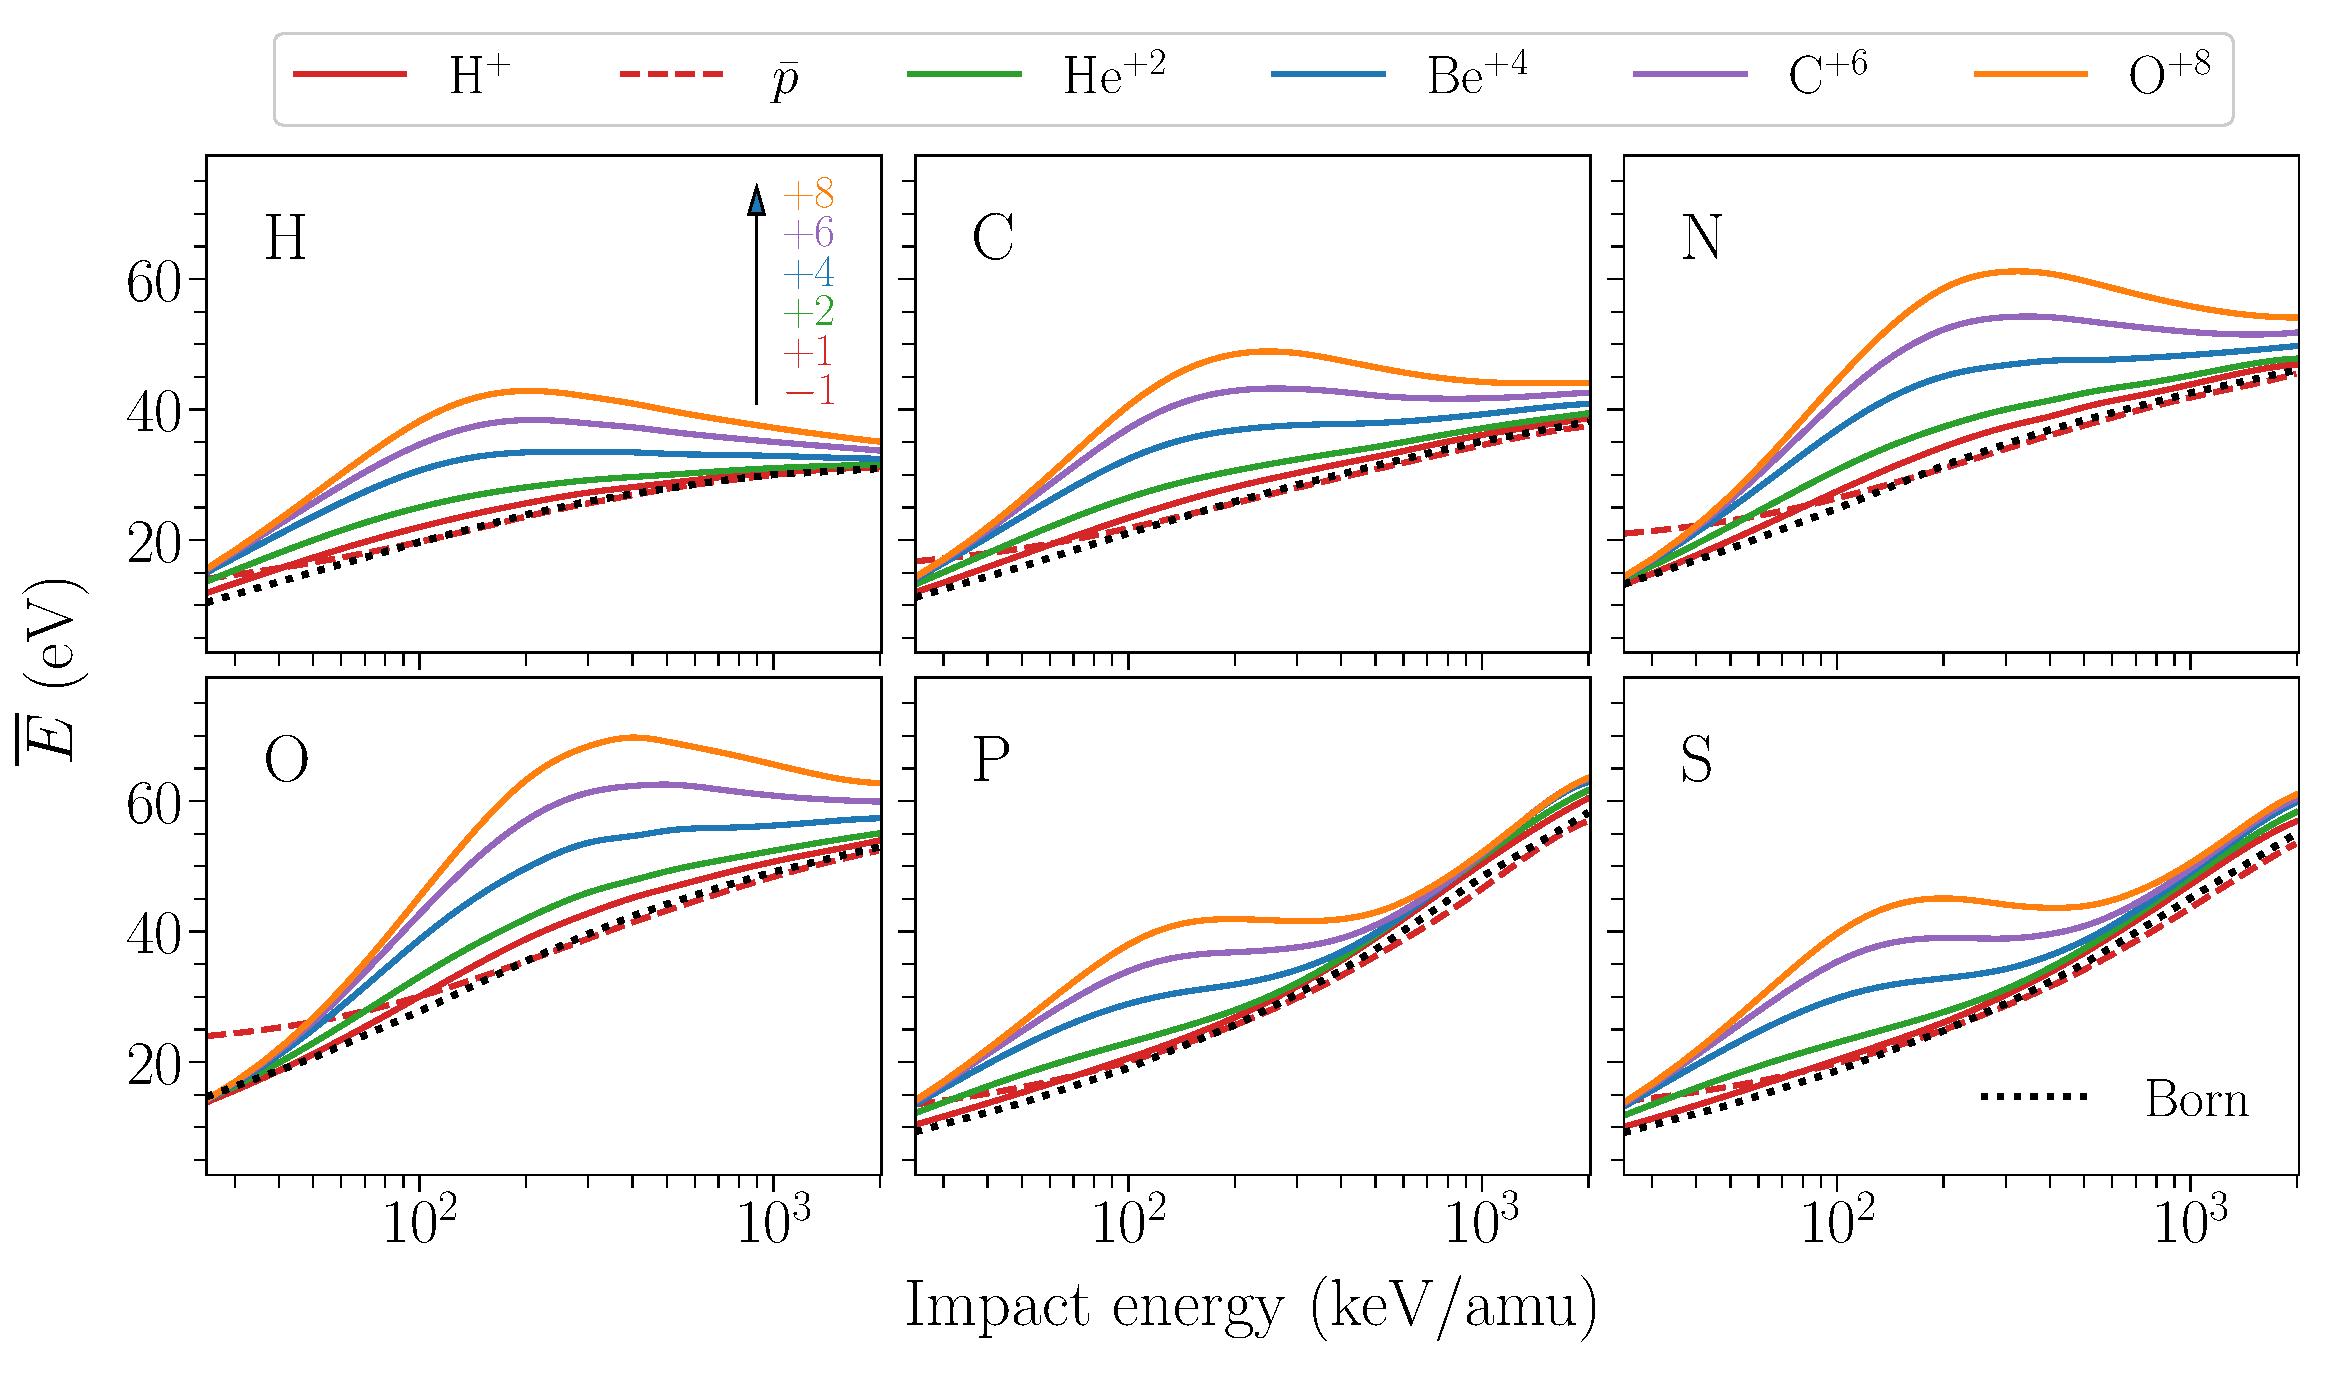
\includegraphics[width=0.9\textwidth]{figuras/ener_mean.eps}
\caption{Mean emitted energy distribution for ionization by impact of
multicharged ions, given by Eq.~(\ref{40}). Dashed lines for $\bar{p}$,
solid lines for ion charges $+1$, $+2$, $+4$, $+6$ and $+8$,
as indicated.}
\label{fig:emittedener}
\end{figure*} 

The mean emitted electron energies $\overline{E}_{\alpha}$ for H, C, N, 
O, P and S are shown in Fig.~\ref{fig:emittedener}. The range of impact 
velocities was shortened to $v=10$ a.u. due to numerical limitations 
in the spherical harmonics expansion of Eq.~(\ref{eq:contwave}). 
As the impact velocity $v$ increases, so do $\langle E_{\alpha}\rangle$
and $l_{\max}$, which results in the inclusion of very oscillatory 
functions in the integrand. Furthermore, the integrand of
$\langle E_{\alpha}\rangle$ includes the kinetic energy $E$
(see Eq.~(\ref{40})), which cancels the small energy region and 
reinforces the large values, making the result more sensible to large
angular momenta. Regardless, for $v>10$ a.u., the first Born 
approximation holds.

In Fig.~\ref{fig:emittedener}, we estimate $\overline{E}_{\alpha}$ of
the emitted electron in the 0.5--2.7 a.u. energy range, or equivalently 
from 15 to 70 eV, for all the targets. Our results agree with the 
experimental findings~\cite{surdutovic2018}. As can be noted in the 
figure, the mean energy value is surprisingly sensible to the 
projectile charge $Z$, which can duplicate the proton results in the 
intermediate region, i.e. 100--400 keV/amu. The effect observed can be 
attributed to the depletion caused by the multicharged ions to the 
yields of low energy electrons. This behavior cannot be found in the 
first Born approximation, where the $Z^2$ law cancels the $Z$ dependence
in Eq.~(\ref{40}). At high energies, $\overline{E}_{\alpha}$ tends to a 
universal value for all ions, as can be seen in Fig.~\ref{fig:emittedener}.


%%%%%%%%%%%%%%%%%%%%%%%%%%%%%%%%%%%%%%%%%%%%%%%%%%%%%%%%%%%%%%%%%%%%%%%%
\subsection{Emitted electron angles}
\label{subsec:meanang}
%%%%%%%%%%%%%%%%%%%%%%%%%%%%%%%%%%%%%%%%%%%%%%%%%%%%%%%%%%%%%%%%%%%%%%%%

As mentioned before, secondary electrons contribute to the total damage. 
Then, not only is the ejection energy important but also the angle 
of emission. Once again, we can consider the single differential cross 
section in terms of the ejected electron solid angle $\Omega$, 
$d\sigma_{\alpha,nl}/d\Omega$, to be expressed as a distribution function, 
and the mean angle $\overline{\theta}_{\alpha}$ can be defined as
\begin{equation}
\overline{\theta}_{\alpha}=\frac{\langle\theta_{\alpha}\rangle}
{\langle 1\rangle}=\frac{1}{\sigma_{\alpha}}\sum\limits_{nl}
\int d\Omega\,\theta\,\frac{d\sigma_{\alpha,nl}}{d\Omega}
\end{equation}

\begin{figure*}[t!]
\centering
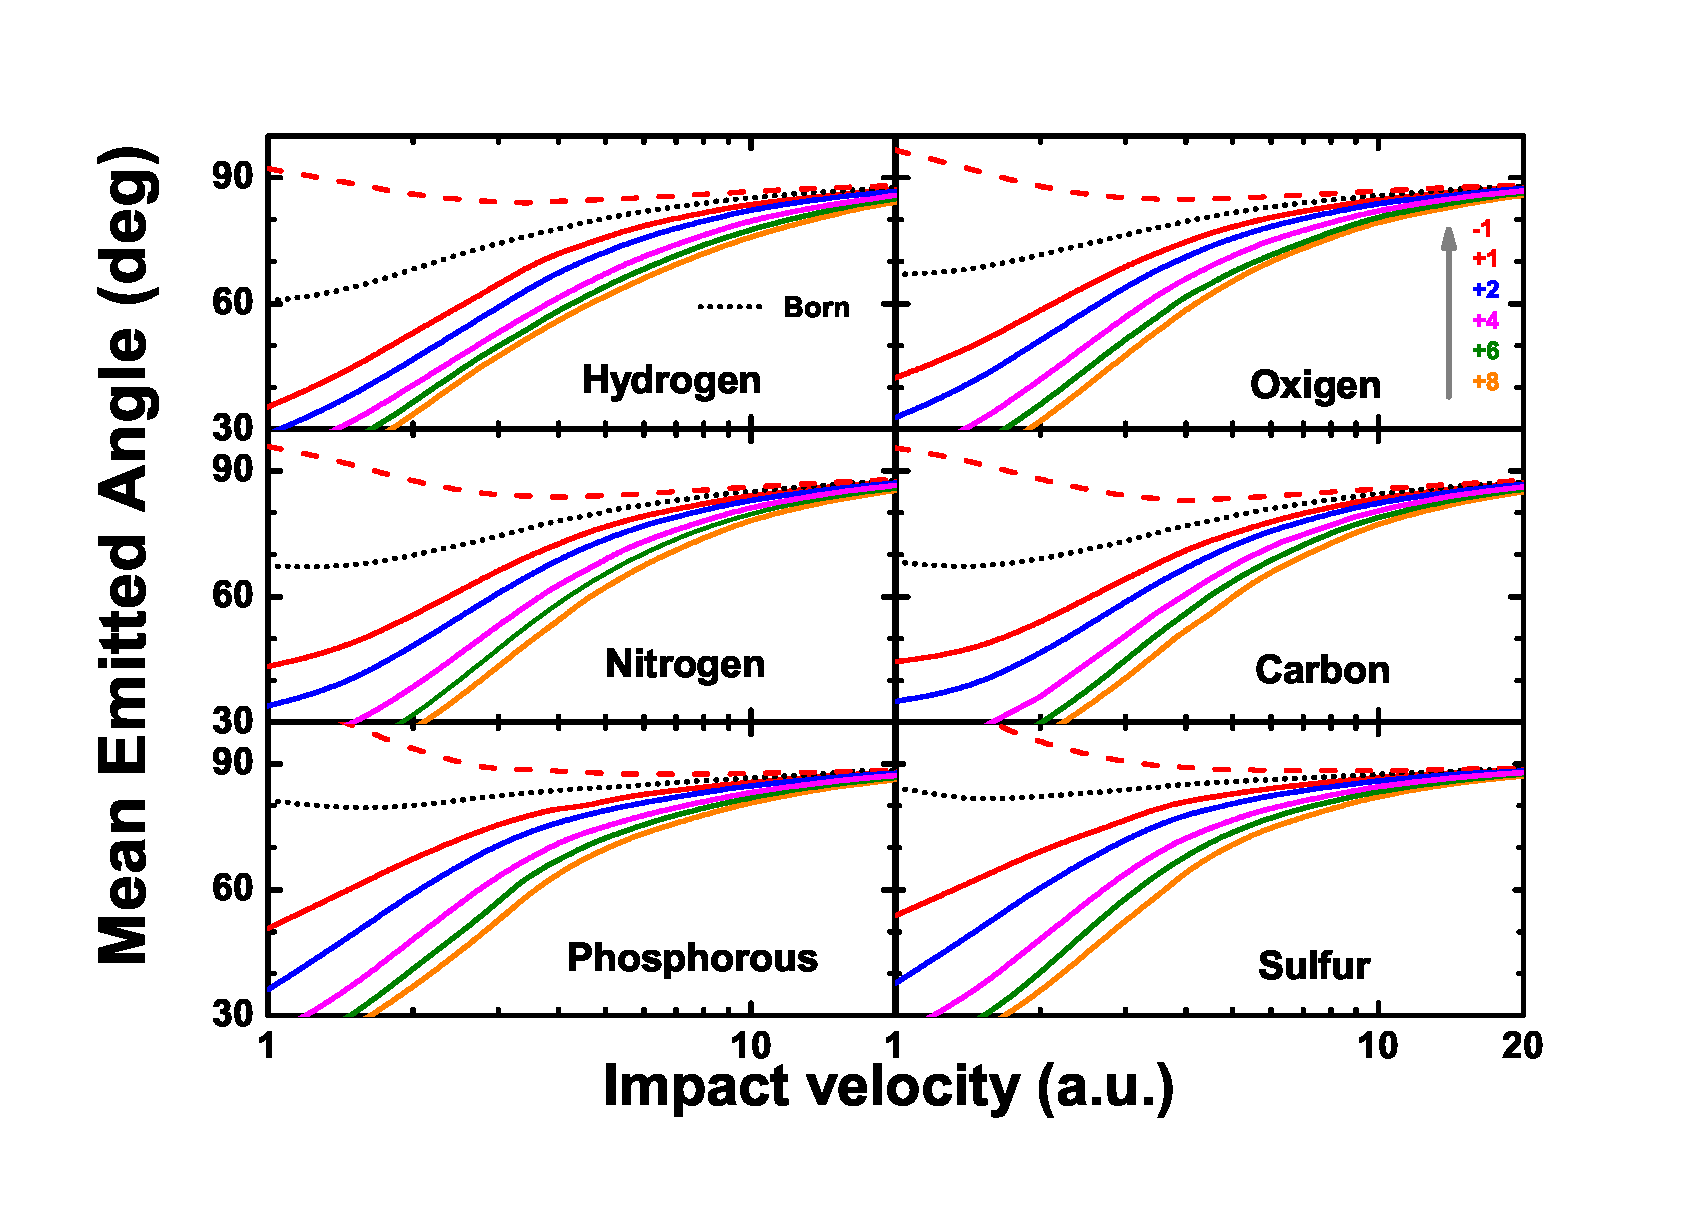
\includegraphics[width=0.75\textwidth]{figuras/Fig_finales/fig6.eps}
%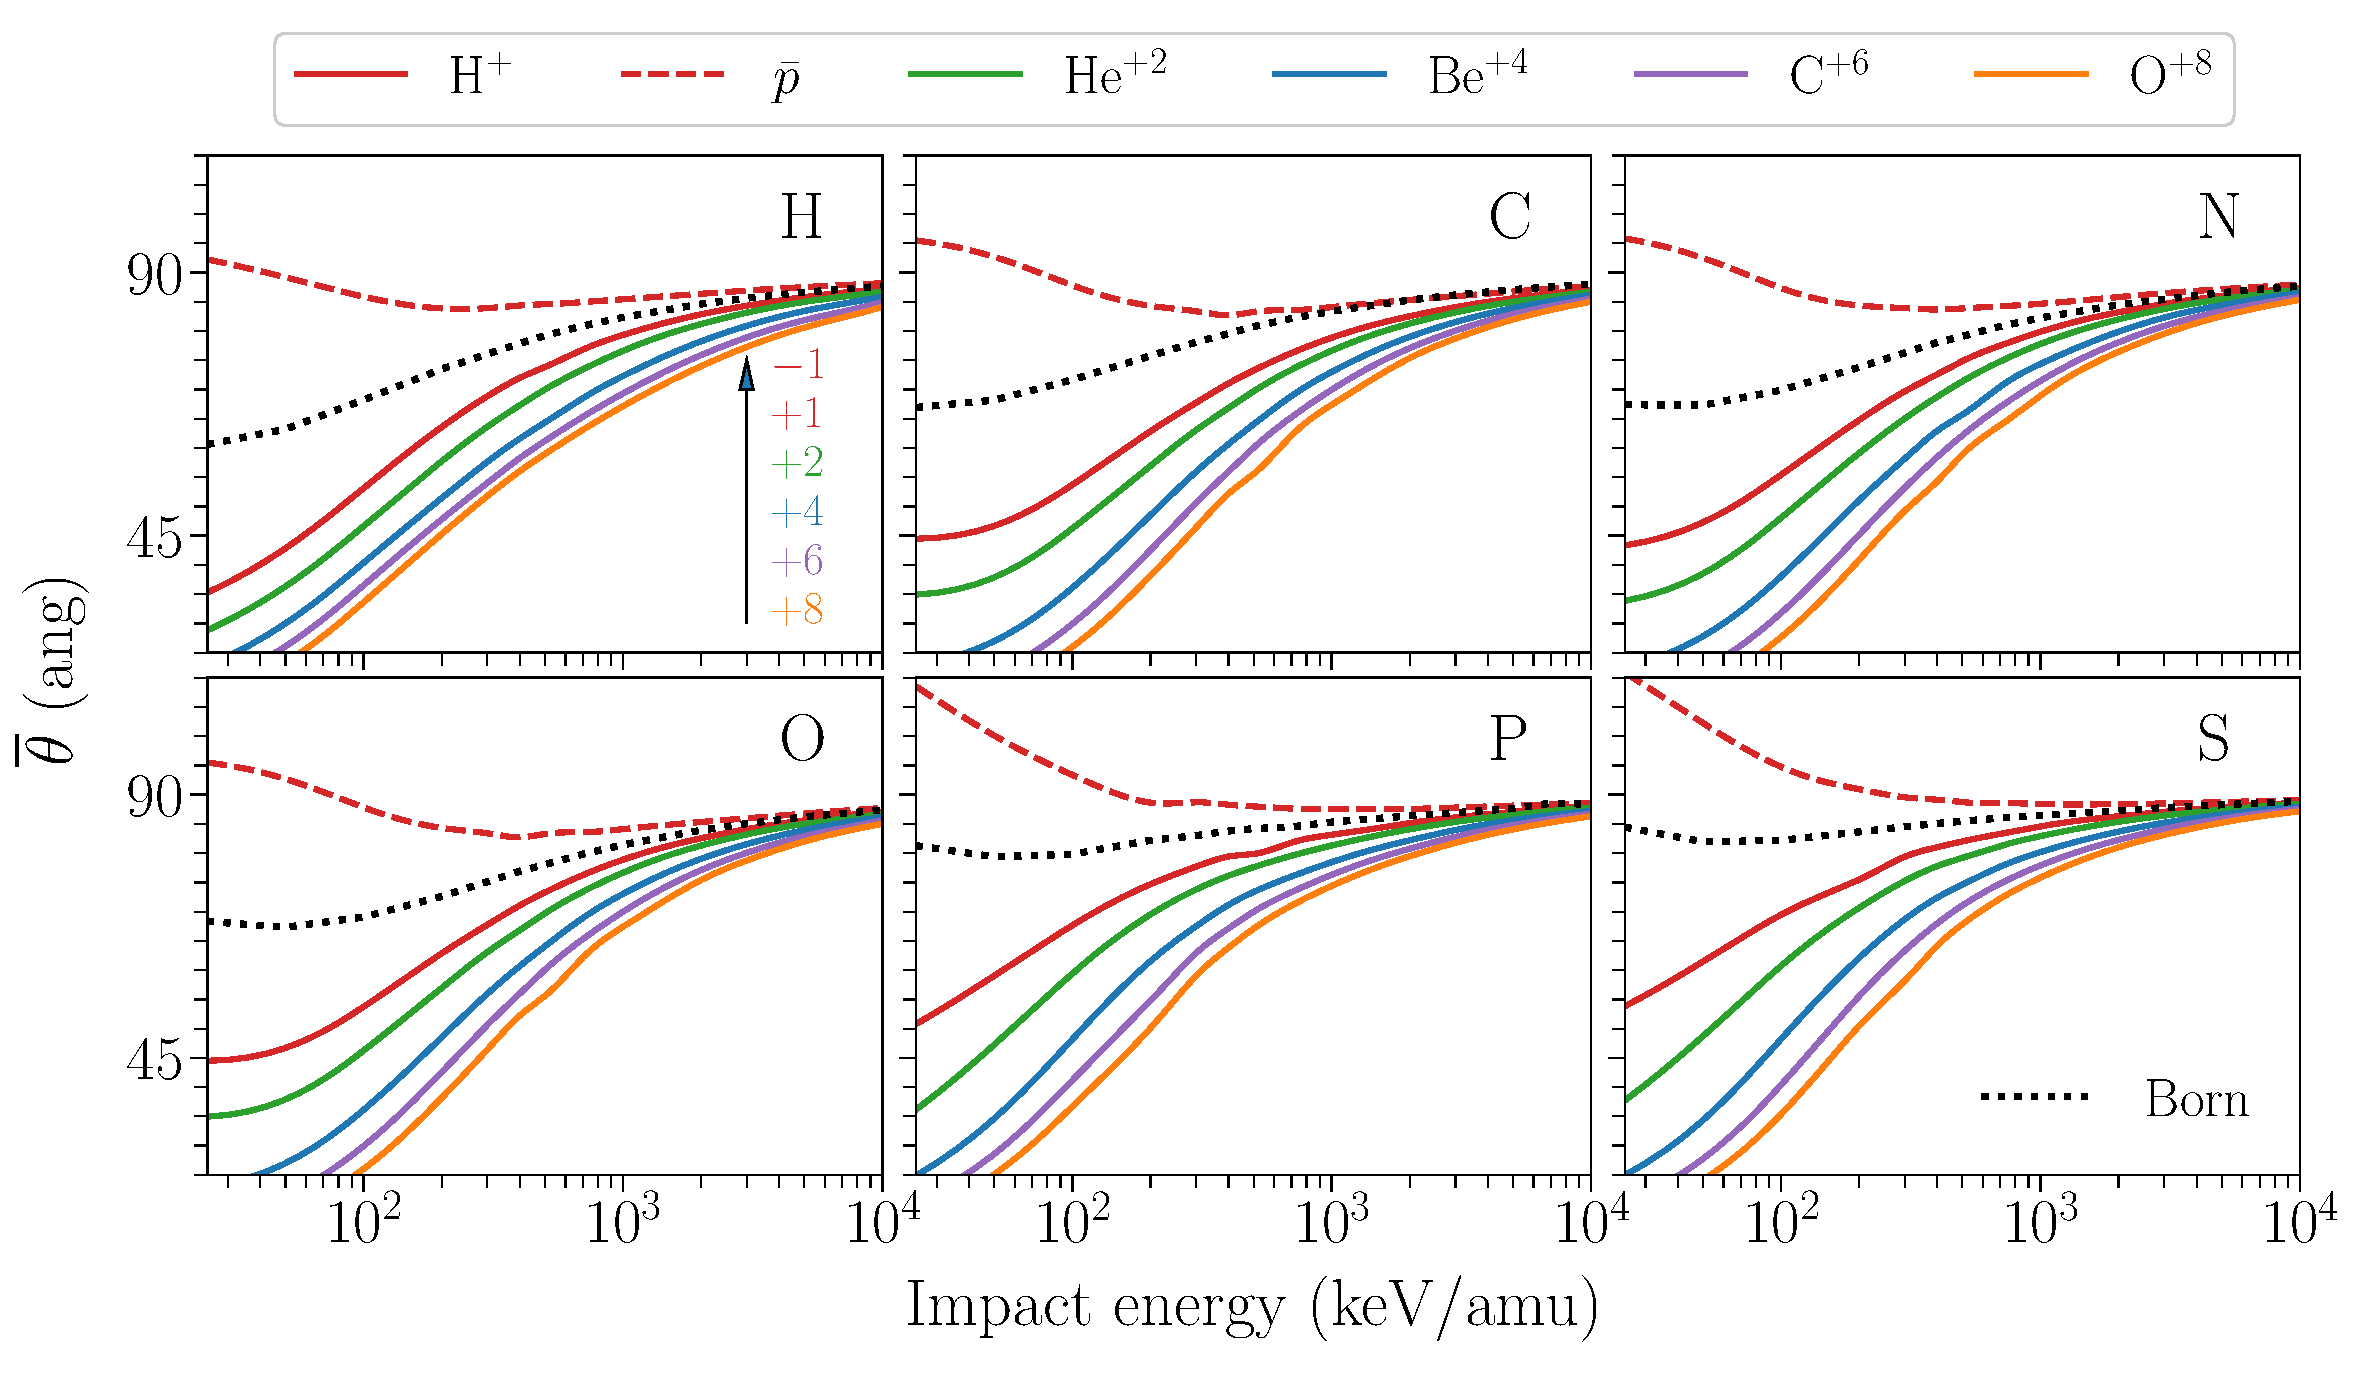
\includegraphics[width=0.9\textwidth]{figuras/ang_mean.eps}
\caption{Mean emitted angle distribution for ionization by impact of
multicharged ions.}
\label{fig:emittedang}
\end{figure*} 

The mean emitted electron angles $\overline{\theta}_{\alpha}$ for the 
six atoms of interest are shown in Fig.~\ref{fig:emittedang}, and an 
important dependence of $\overline{\theta}_{\alpha}$ with $Z$ is 
observed. Once again, this effect is not observed in the first Born 
approximation. It is a general belief~\cite{Rudd1992} that the 
angular dispersion of emitted electrons are nearly isotropic. This 
behavior is caused by the insignificant angular anisotropy of 
sub--50--eV yield. 
A typical value for the ejection angle considered in the literature is 
$\overline{\theta}_{\alpha}\sim 70\degree$~\cite{surdutovic2018}, and 
it is quite correct in the range of validity of the first Born 
approximation for any target. But, when a distorted wave approximation 
is used, $\overline{\theta}_{\alpha}$ decreases substantially with $Z$ 
in the intermediate energy region, as observed in Fig.~\ref{fig:emittedang}. 
For example, for C$^{+6}$ impact, the Bragg peak occurs at 0.3 MeV/amu, 
where $\overline{\theta}_{\alpha}$, computed with the CDW method, is 
about half of the value obtained with the first Born approximation. 
This correction closes the damage to the forward direction.

We can attribute this forward direction correction to the capture to 
the continuum effect; the larger the charge $Z$, the smaller 
$\overline{\theta}$ will be. Of course, this effect only holds at 
intermediate energies and not at high impact energies, where the Born 
approximation rules. One illustrative observation is the behavior of 
antiprotons: the projectile in this case repels the electrons, being
$\overline{\theta}_{\alpha}\sim 90\degree$.
Note the opposite effect of proton and antiprotons; they run one 
opposite to the other, as compared with the first Born approximation,
constituting an angular Barkas effect.


%%%%%%%%%%%%%%%%%%%%%%%%%%%%%%%%%%%%%%%%%%%%%%%%%%%%%%%%%%%%%%%%%%%%%%%%
\section{Ionization of Molecules}
%%%%%%%%%%%%%%%%%%%%%%%%%%%%%%%%%%%%%%%%%%%%%%%%%%%%%%%%%%%%%%%%%%%%%%%%
\subsection{The stoichiometric model}
%%%%%%%%%%%%%%%%%%%%%%%%%%%%%%%%%%%%%%%%%%%%%%%%%%%%%%%%%%%%%%%%%%%%%%%%

Lets us consider a molecule $M$ composed by $n_{\alpha}$ atoms of the
element $\alpha$, the SSM approaches the total ionization cross section 
of the molecule $\sigma_{M}$ as a sum of ionization cross sections of 
the isolated atoms $\sigma_{\alpha}$ weighted by $n_{\alpha}$, 
\begin{equation}
 \sigma_{M}=\sum\limits_{\alpha}n_{\alpha}\sigma_{\alpha}\,.  
 \label{eq:sumion}
\end{equation}
We classified the molecular targets of our interest in three families: 
CH, CHN and DNA, as in Table~\ref{tab:families}.

\begin{table}[H]
\begin{center}
\begin{tabular}{|p{0.06\textwidth}|p{0.6\textwidth}|}
\hline
\multirow{2}{*}{CH} 
      & CH$_4$ (methane), C$_2$H$_2$ (acetylene), C$_2$H$_4$ (ethene), \\
      & C$_2$H$_6$ (ethane), C$_6$H$_6$ (benzene) \\
\hline
\multirow{2}{*}{CHN} 
      & C$_5$H$_5$N (pyridine), C$_4$H$_4$N$_2$ (pyrimidine), \\ 
      & C$_2$H$_7$N (dimenthylamine), CH$_5$N (monomethylamine) \\
\hline
\multirow{4}{*}{DNA} 
      & C$_5$H$_5$N$_5$ (adenine), C$_4$H$_5$N$_3$O (cytosine), \\
      & C$_5$H$_5$N$_5$O (guanine), C$_5$H$_6$N$_2$O$_2$ (thymine), \\
      & C$_4$H$_4$N$_2$O$_2$ (uracil), C$_4$H$_8$O (THF), \\
      & C$_5$H$_{10}$O$_5$P (DNA backbone), 
        C$_{20}$H$_{27}$N$_7$O$_{13}$P$_2$ 
(dry DNA) \\
\hline
\end{tabular}
\caption{Molecular targets studied in this work, classified in three 
families.}
\label{tab:families}
\end{center}
\end{table}

In Fig.~\ref{fig:crossDNA_1}, we report the total ionization cross 
sections by the impact of multicharged ions for adenine, cytosine, 
guanine and thymine. For adenine, the agreement with the experimental 
data available~\cite{iriki2011} is very good. To the best of our 
knowledge, there are not experimental data on ion--collision ionization 
for the rest of the molecules. We included electron impact 
measurements~\cite{rahman2016} with the corresponding equivelocity 
conversion for incident energies higher than 300~eV. In this region, 
the proton and electron cross section should converge. Although the 
electron impact measurements are above our findings for all the 
molecular targets, it is worth stating that our results agree very well 
with other electron impact theoretical 
predictions~\cite{mozejko2003,tan2018}. 

\begin{figure*}[t!]
\centering
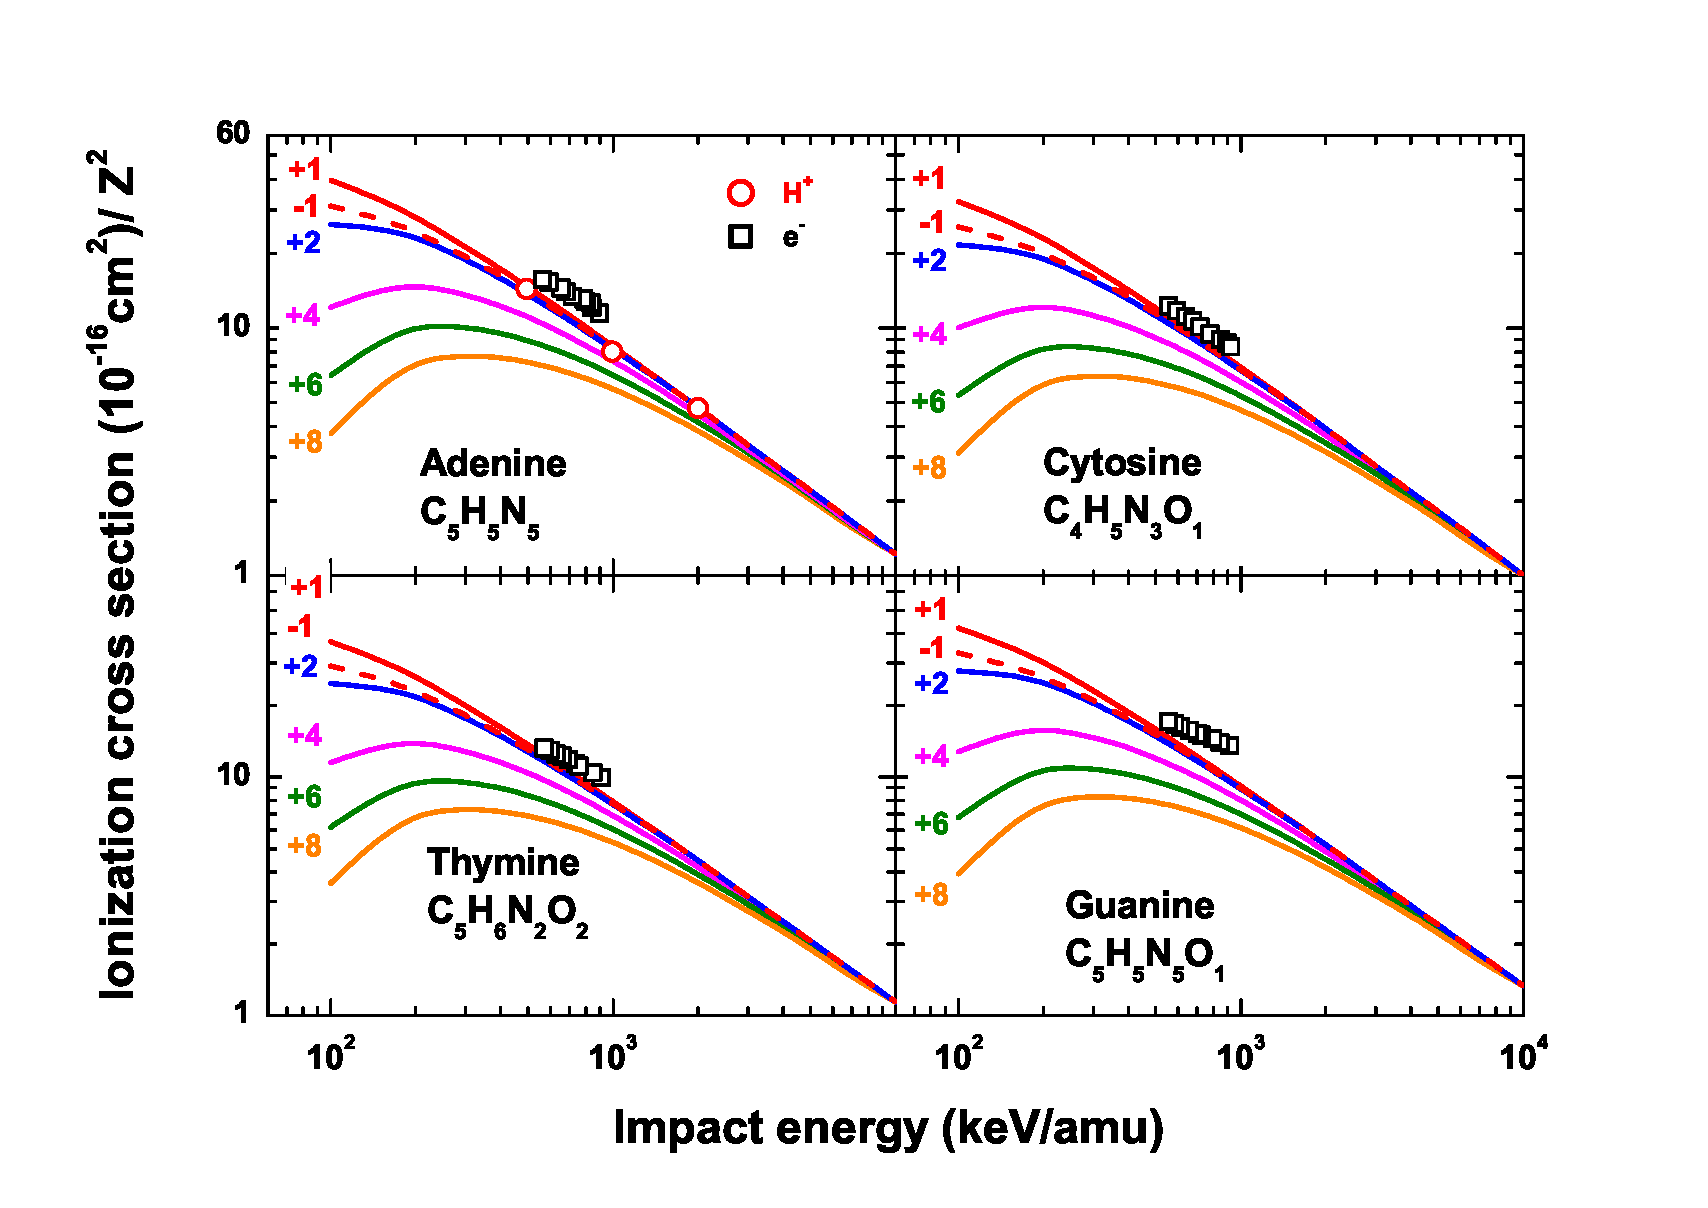
\includegraphics[width=0.75\textwidth]{figuras/Fig_finales/fig2.eps}
%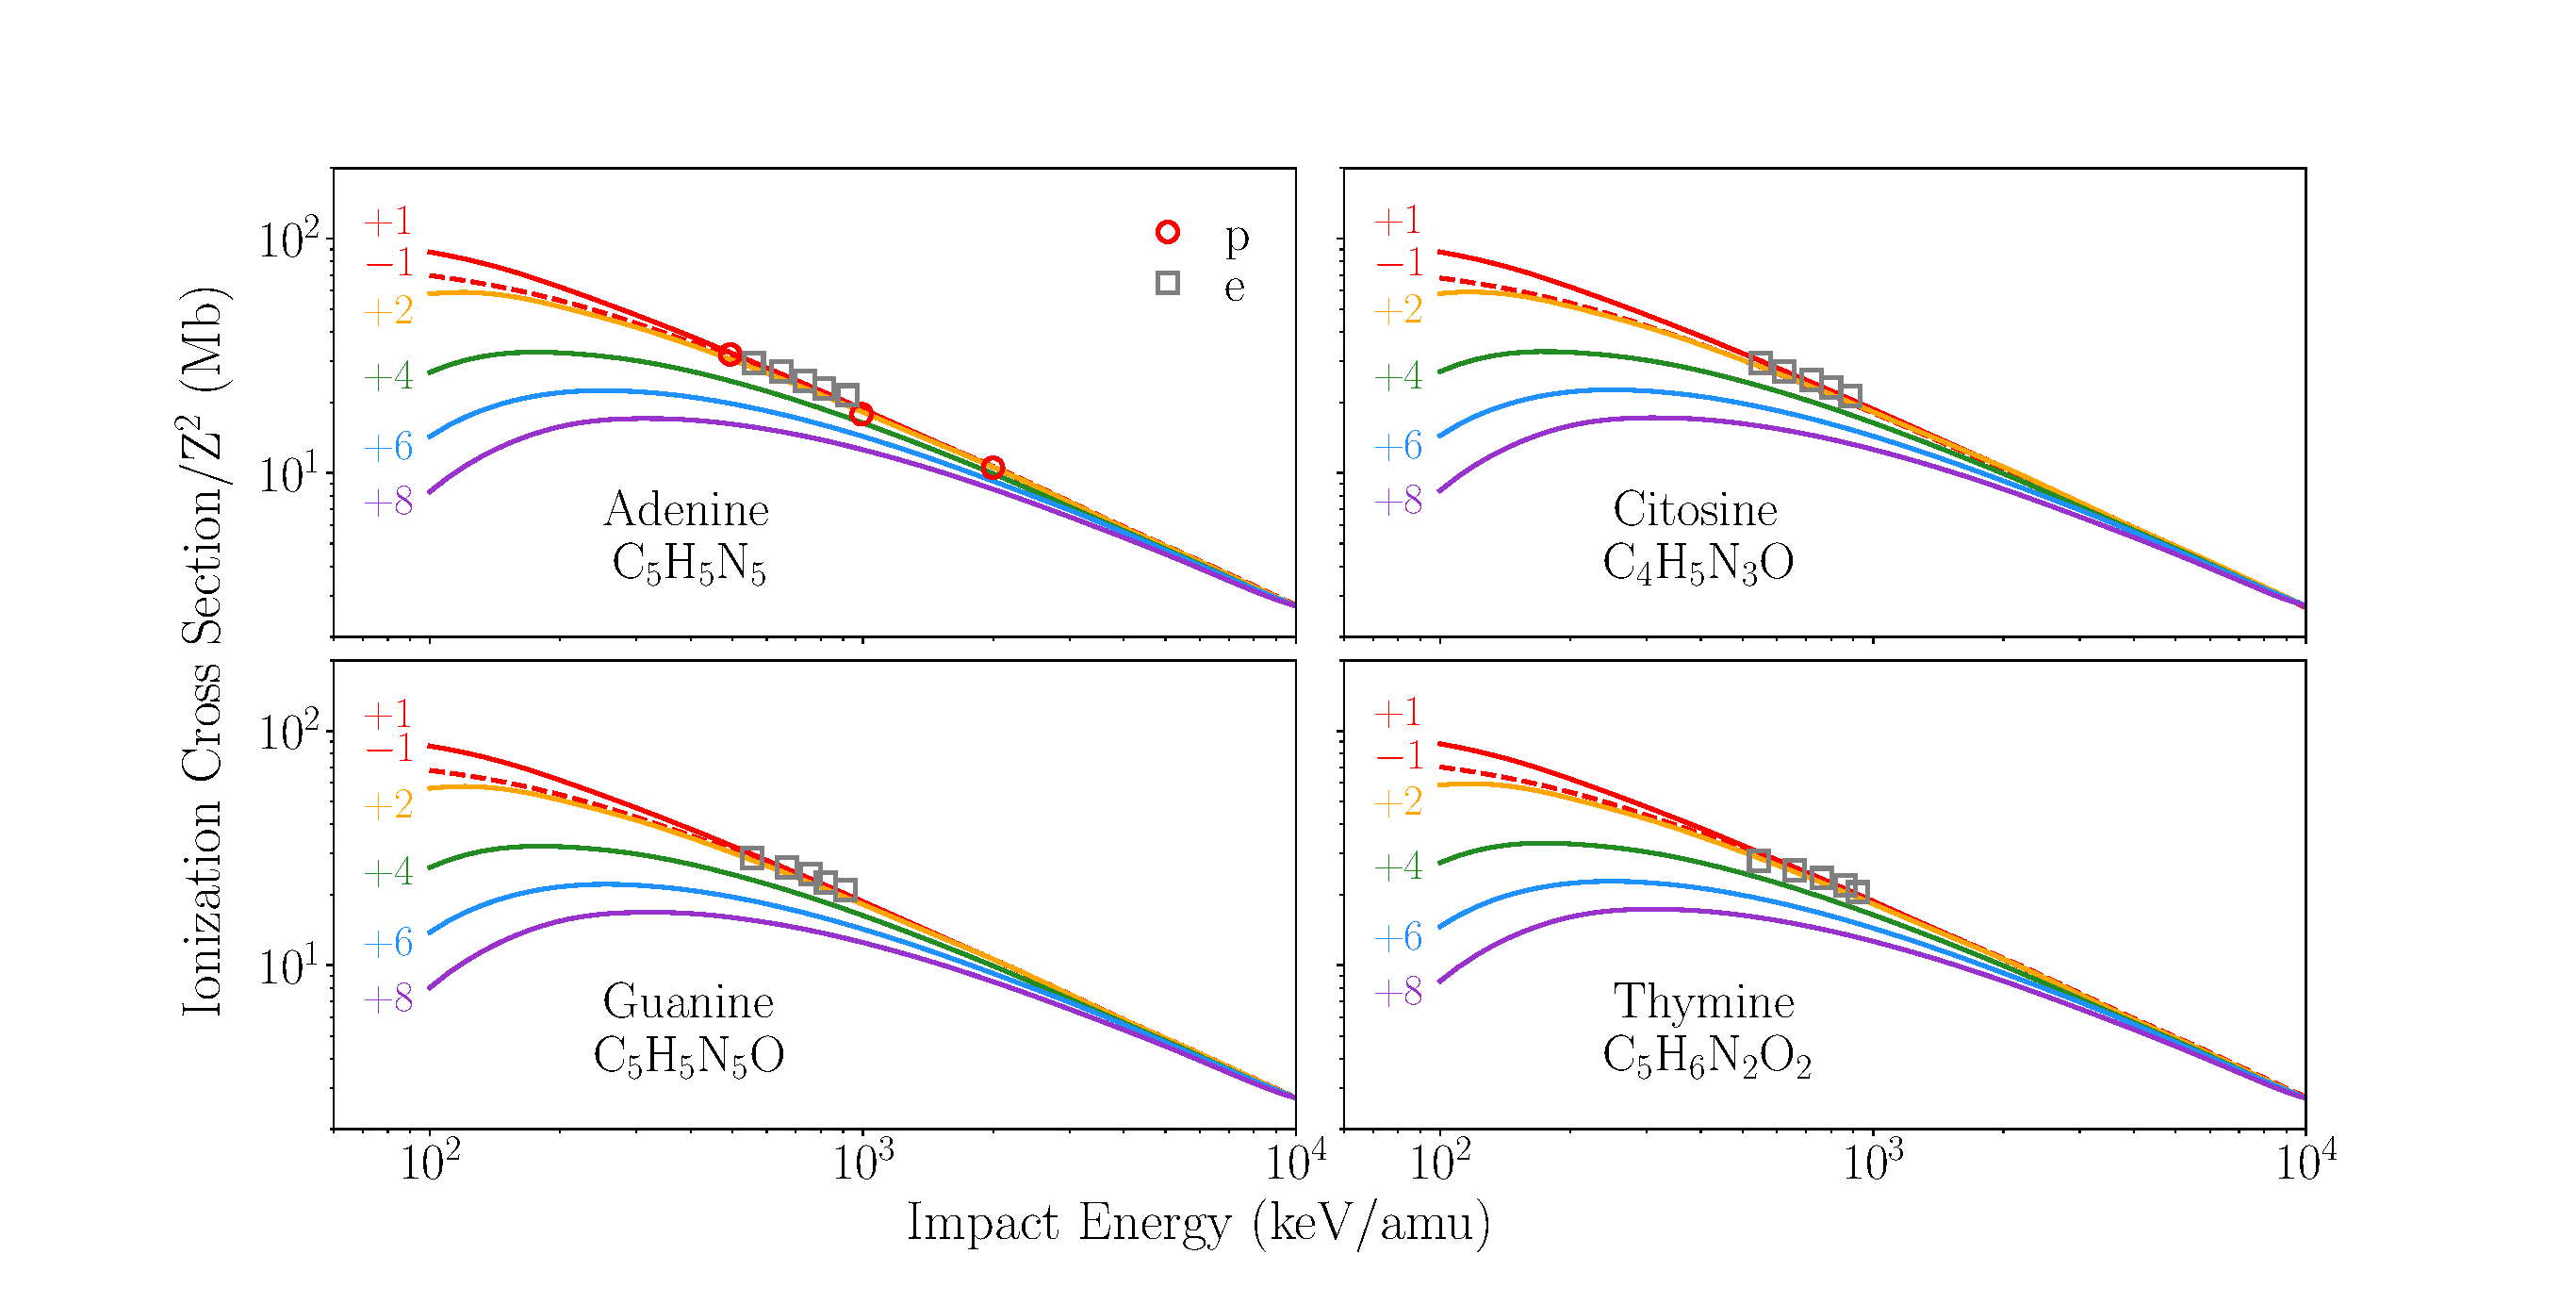
\includegraphics[width=0.9\textwidth]{figuras/adn1.eps}
\caption{Reduced CDW ionization cross section by impact of multicharged 
ions. Experiments: \mbox{\Large$\circ$}~\cite{iriki2011} for proton 
impact and $\square$~\cite{rahman2016} for electron impact with 
equivelocity conversion.}
\label{fig:crossDNA_1}
\end{figure*} 

Our results for uracil, DNA backbone, pyrimidine and THF are displayed 
in Fig.~\ref{fig:crossDNA_2}. For uracil, the agreement with the 
experimental proton impact measurements by 
Itoh~{\it et al.}~\cite{itoh2013} is good.
However, for the same target, our theory fails by a factor of two for 
the experimental ionization values by the impact of 
C$^{+4}$, O$^{+6}$ and O$^{+8}$ ions~\cite{agnihotri2012,agnihotri2013}.
Nonetheless, it should be stated that our theoretical results coincide 
with calculations by Champion, Rivarola and 
collaborators~\cite{agnihotri2012,champion2012}, which may indicate a 
possible misstep of the experiments. 
For pyrimidine, we show comparison of our results with experimental data
for proton~\cite{wolff2014} and electron~\cite{bug2017} ionization. 
The electron impact measurements 
agree with our calculations for energies higher than 500keV. 
Unexpectedly, the proton impact cross sections are significantly lower 
than our findings. 
The THF molecule results are compared with proton~\cite{wang2016} 
and electron~\cite{bug2017,wolf2019,fuss2009} impact measurements, showing
overall good agreement with our theory. 

\begin{figure*}[t!]
\centering
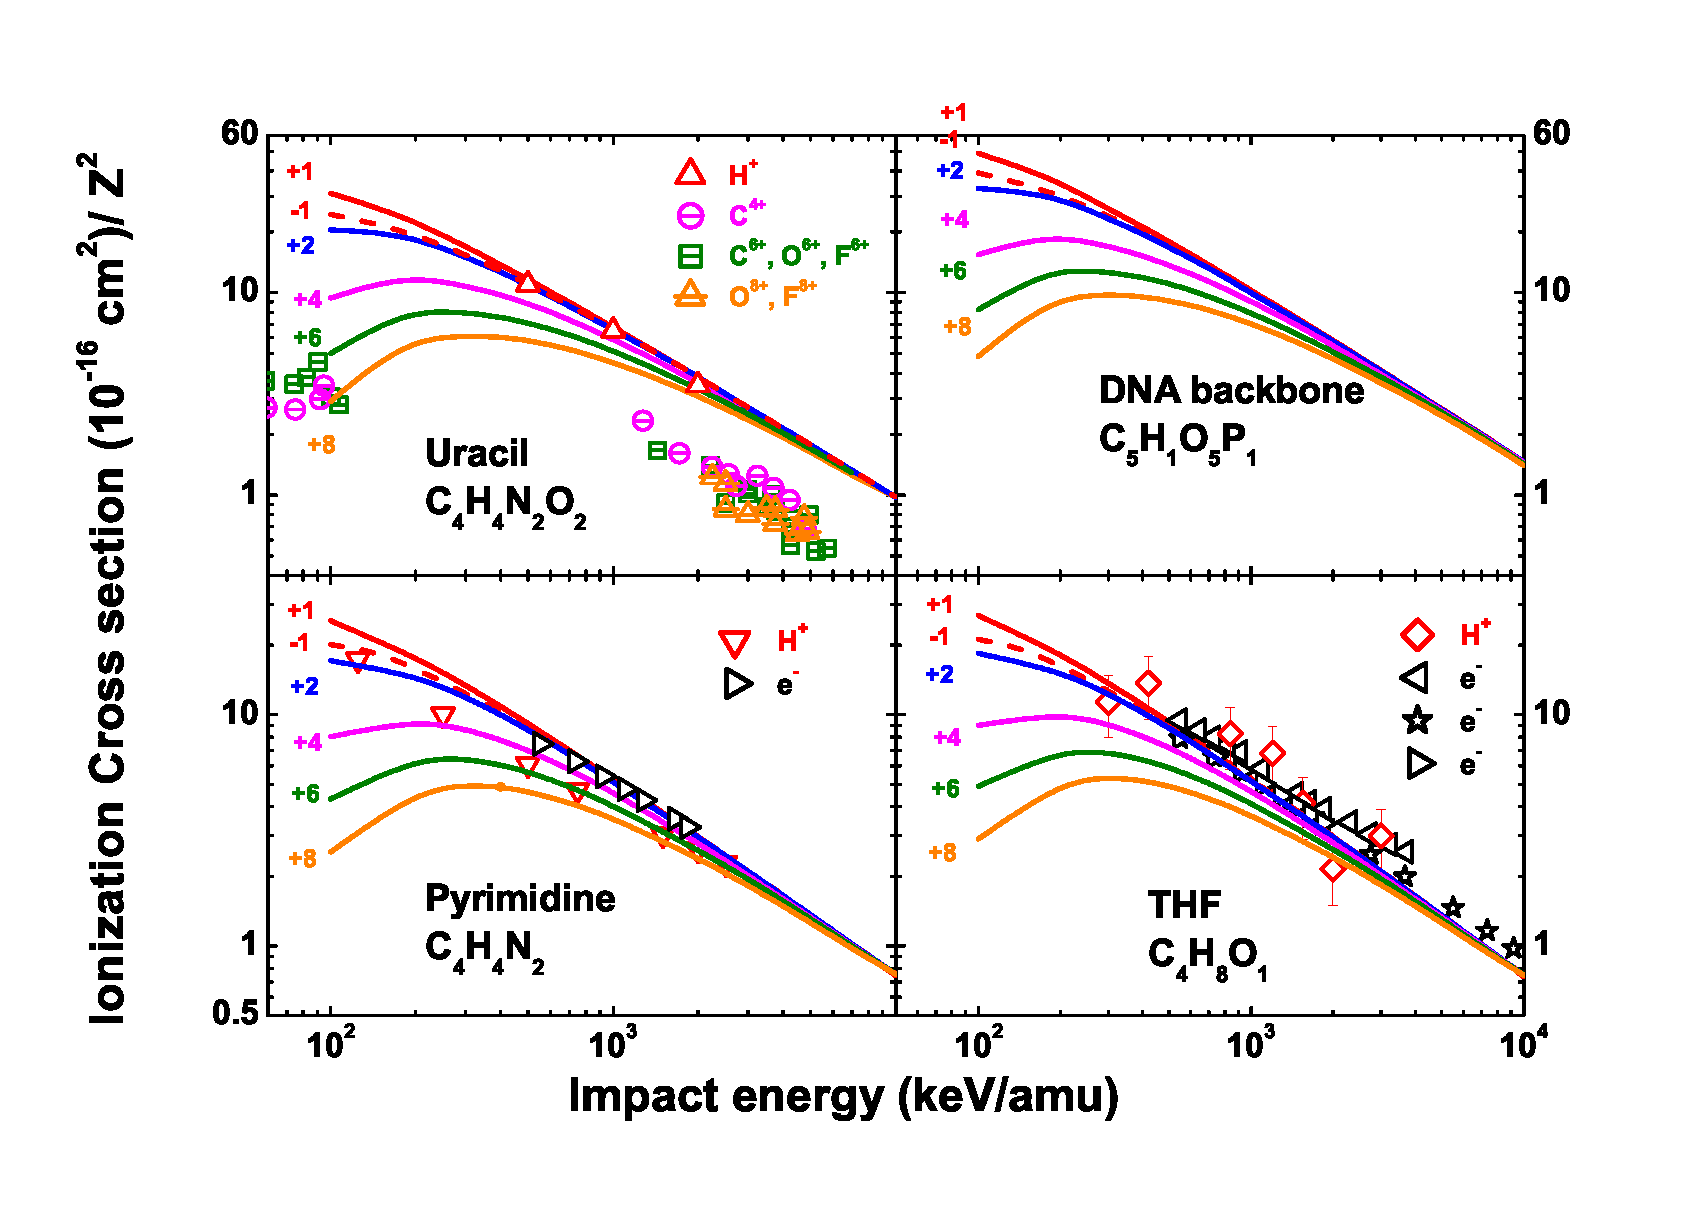
\includegraphics[width=0.75\textwidth]{figuras/Fig_finales/fig3.eps}
%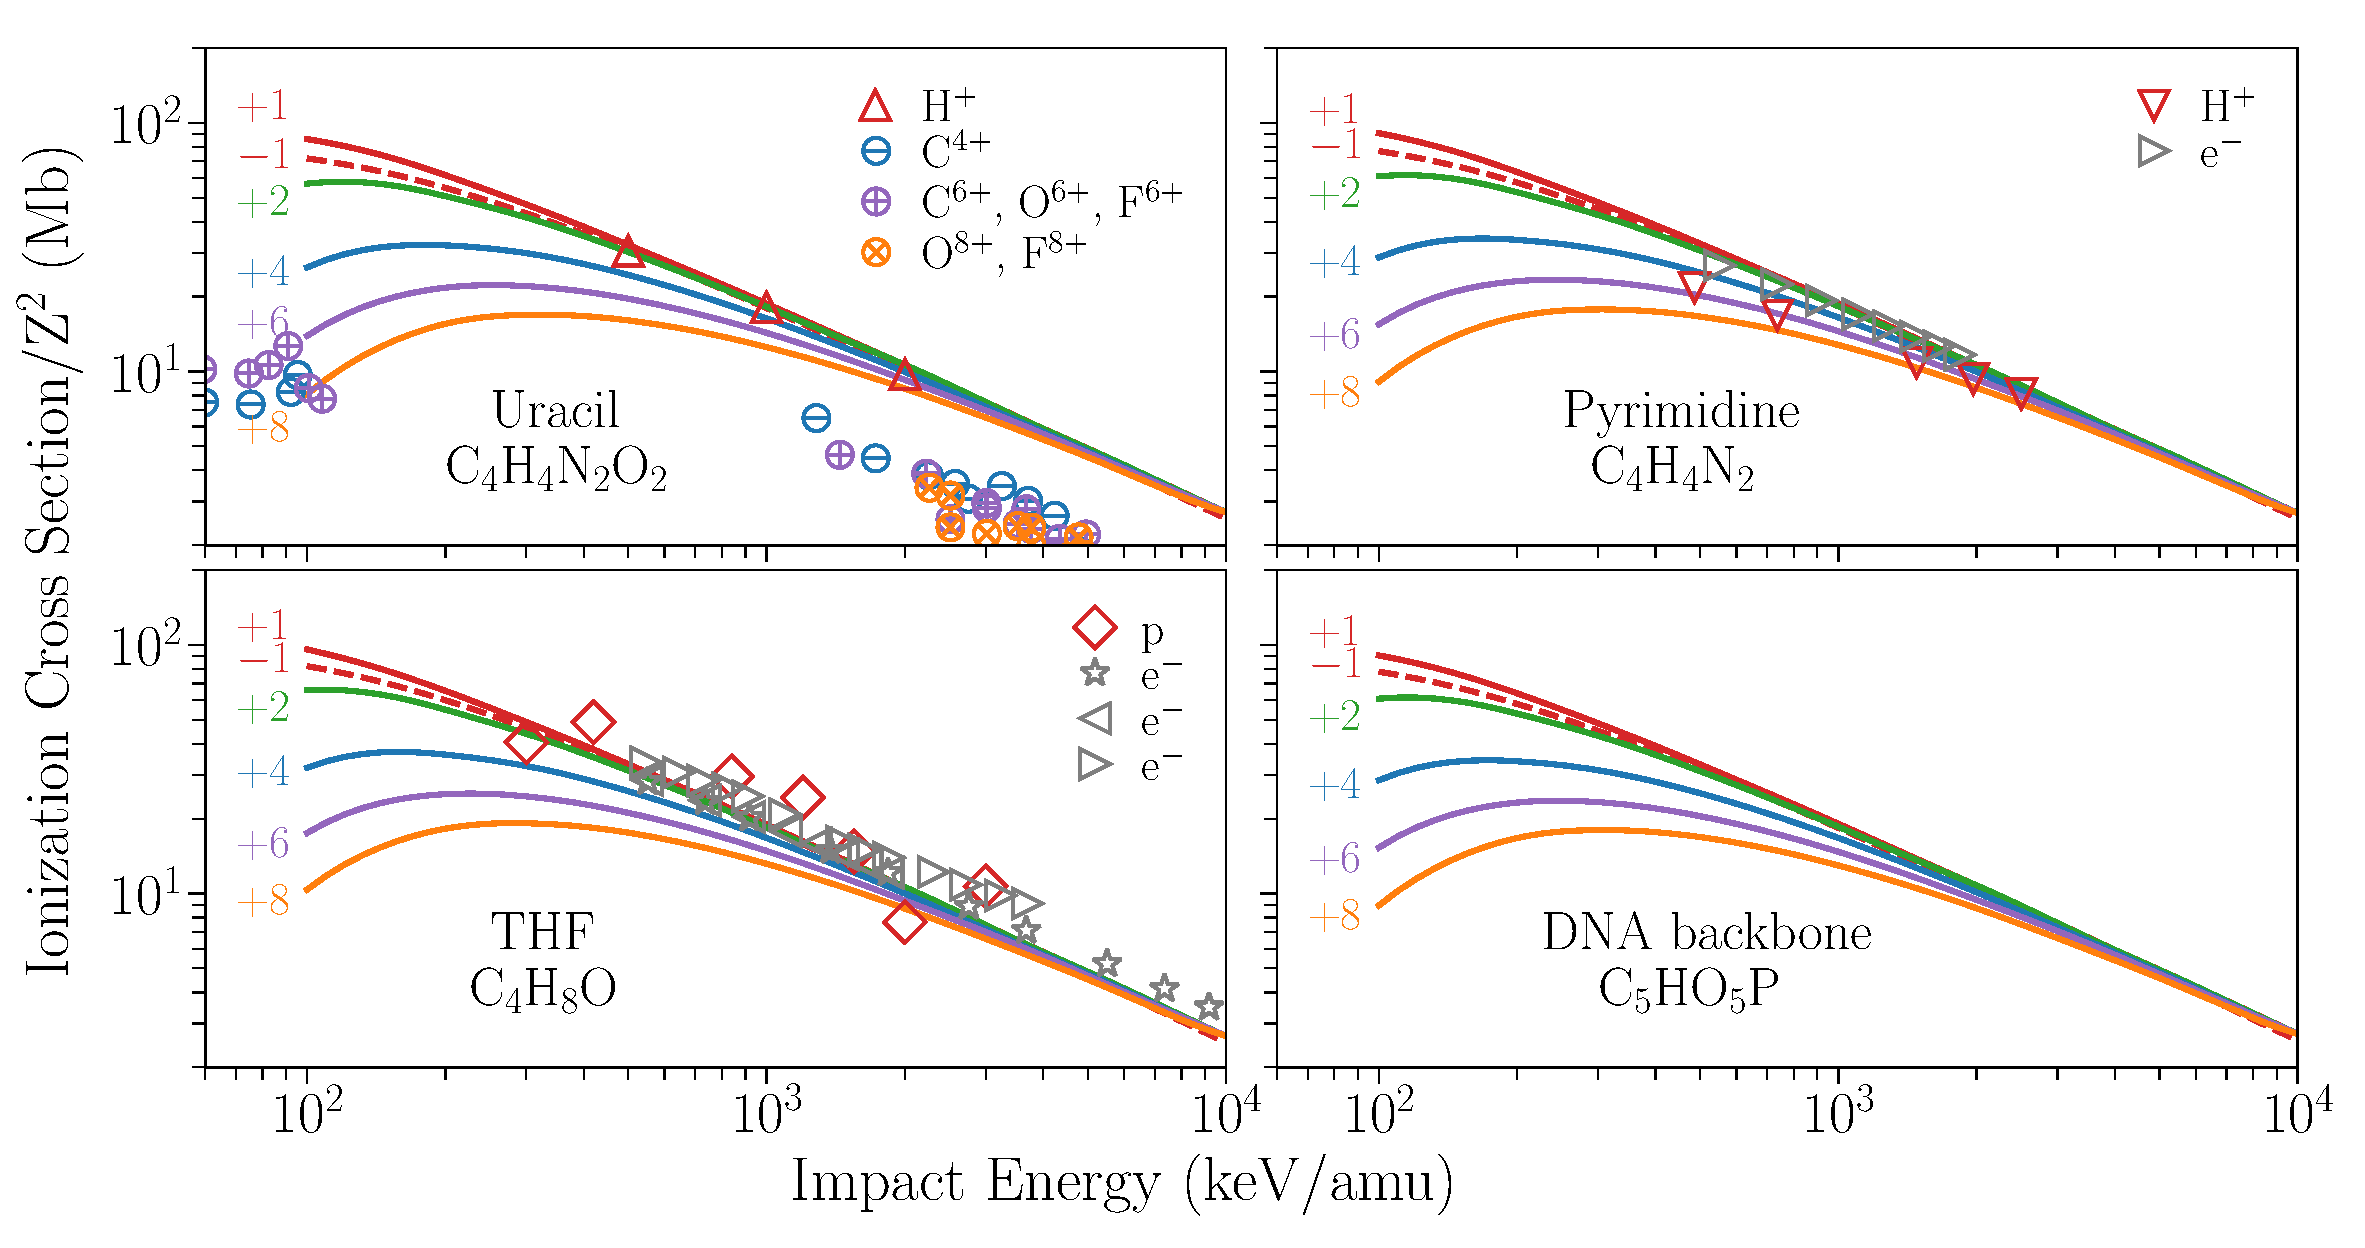
\includegraphics[width=0.9\textwidth]{figuras/adn2.eps}
\caption{Reduced CDW ionization cross section by impact of multicharged 
ions. Experiments: proton impact on $\triangle$ uracil~\cite{itoh2013}, 
$\bigtriangledown$ pyrimidine~\cite{wolff2014} and $\meddiamond$
THF~\cite{wang2016}. Impact of $\ominus$ C$^{+4}$, 
$\boxminus$ C$^{+6}$, O$^{+6}$, F$^{+6}$, and
$\triangle\mkern-14mu-$ O$^{+8}$, F$^{+8}$ on 
uracil~\cite{agnihotri2012,agnihotri2013}. 
Symbols~$\rhd$~\cite{bug2017}, $\lhd$~\cite{wolf2019}, and 
$\medstar$~\cite{fuss2009} for electron impact with equivelocity 
conversion.}
\label{fig:crossDNA_2}
\end{figure*} 

%%%%%%%%%%%%%%%%%%%%%%%%%%%%%%%%%%%%%%%%%%%%%%%%%%%%%%%%%%%%%%%%%%%%%%%%
\subsection{Scaling rule}
\label{subsec:scaling}
%%%%%%%%%%%%%%%%%%%%%%%%%%%%%%%%%%%%%%%%%%%%%%%%%%%%%%%%%%%%%%%%%%%%%%%%
\subsubsection{Toburen rule}
%%%%%%%%%%%%%%%%%%%%%%%%%%%%%%%%%%%%%%%%%%%%%%%%%%%%%%%%%%%%%%%%%%%%%%%%

The first attempt to develop a comprehensive but straightforward 
phenomenological model for electron ejection from large molecules was 
proposed by Toburen and coworkers~\cite{toburen1975,toburen1976}. 
The authors found it convenient to scale the experimental ionization 
cross section in terms of the number of weakly--bound electrons, $n_e$.
For instance, for C, N, O, P and S, this number is the total number of 
electrons minus the K--shell. Following Toburen, the scaled ionization 
cross section per weakly bound electron $\sigma_{e}^T$ is
\begin{equation}
\sigma_{e}^T=\frac{\sigma_{M}}{n_e}\,, 
\label{27} 
\end{equation}
where $n_e=\sum_{\alpha}n_{\alpha}\nu_{\alpha}^T$, and $\nu_{\alpha}^T$ 
are the Toburen numbers given by
\begin{equation}
\nu_{\alpha}^T=\left\{ 
\begin{array}{ll}
1, & \text{for H,} \\
4, & \text{for C,} \\ 
5, & \text{for N and P,} \\ 
6, & \text{for O and S}\,.
\end{array}\right.
\label{eq:nelec} 
\end{equation} 
The Toburen rule can be stated by saying that 
$\sigma_{e}$ is a \textit{universal} parameter independent on the 
molecule, which depends solely on the impact velocity, and holds for 
high impact energies (i.e. 0.25--5 MeV/amu).
These $\nu_{\alpha}^T$ can be interpreted as the number of active 
electrons in the collision. Of course, at very high energies also de 
K--shell electrons will be ionized and these numbers will be different.
A similar dependence with the number of weakly bound electrons was 
found in Ref.~\cite{itoh2013} for proton impact on uracil and adenine.

\begin{figure*}[t!]
\centering
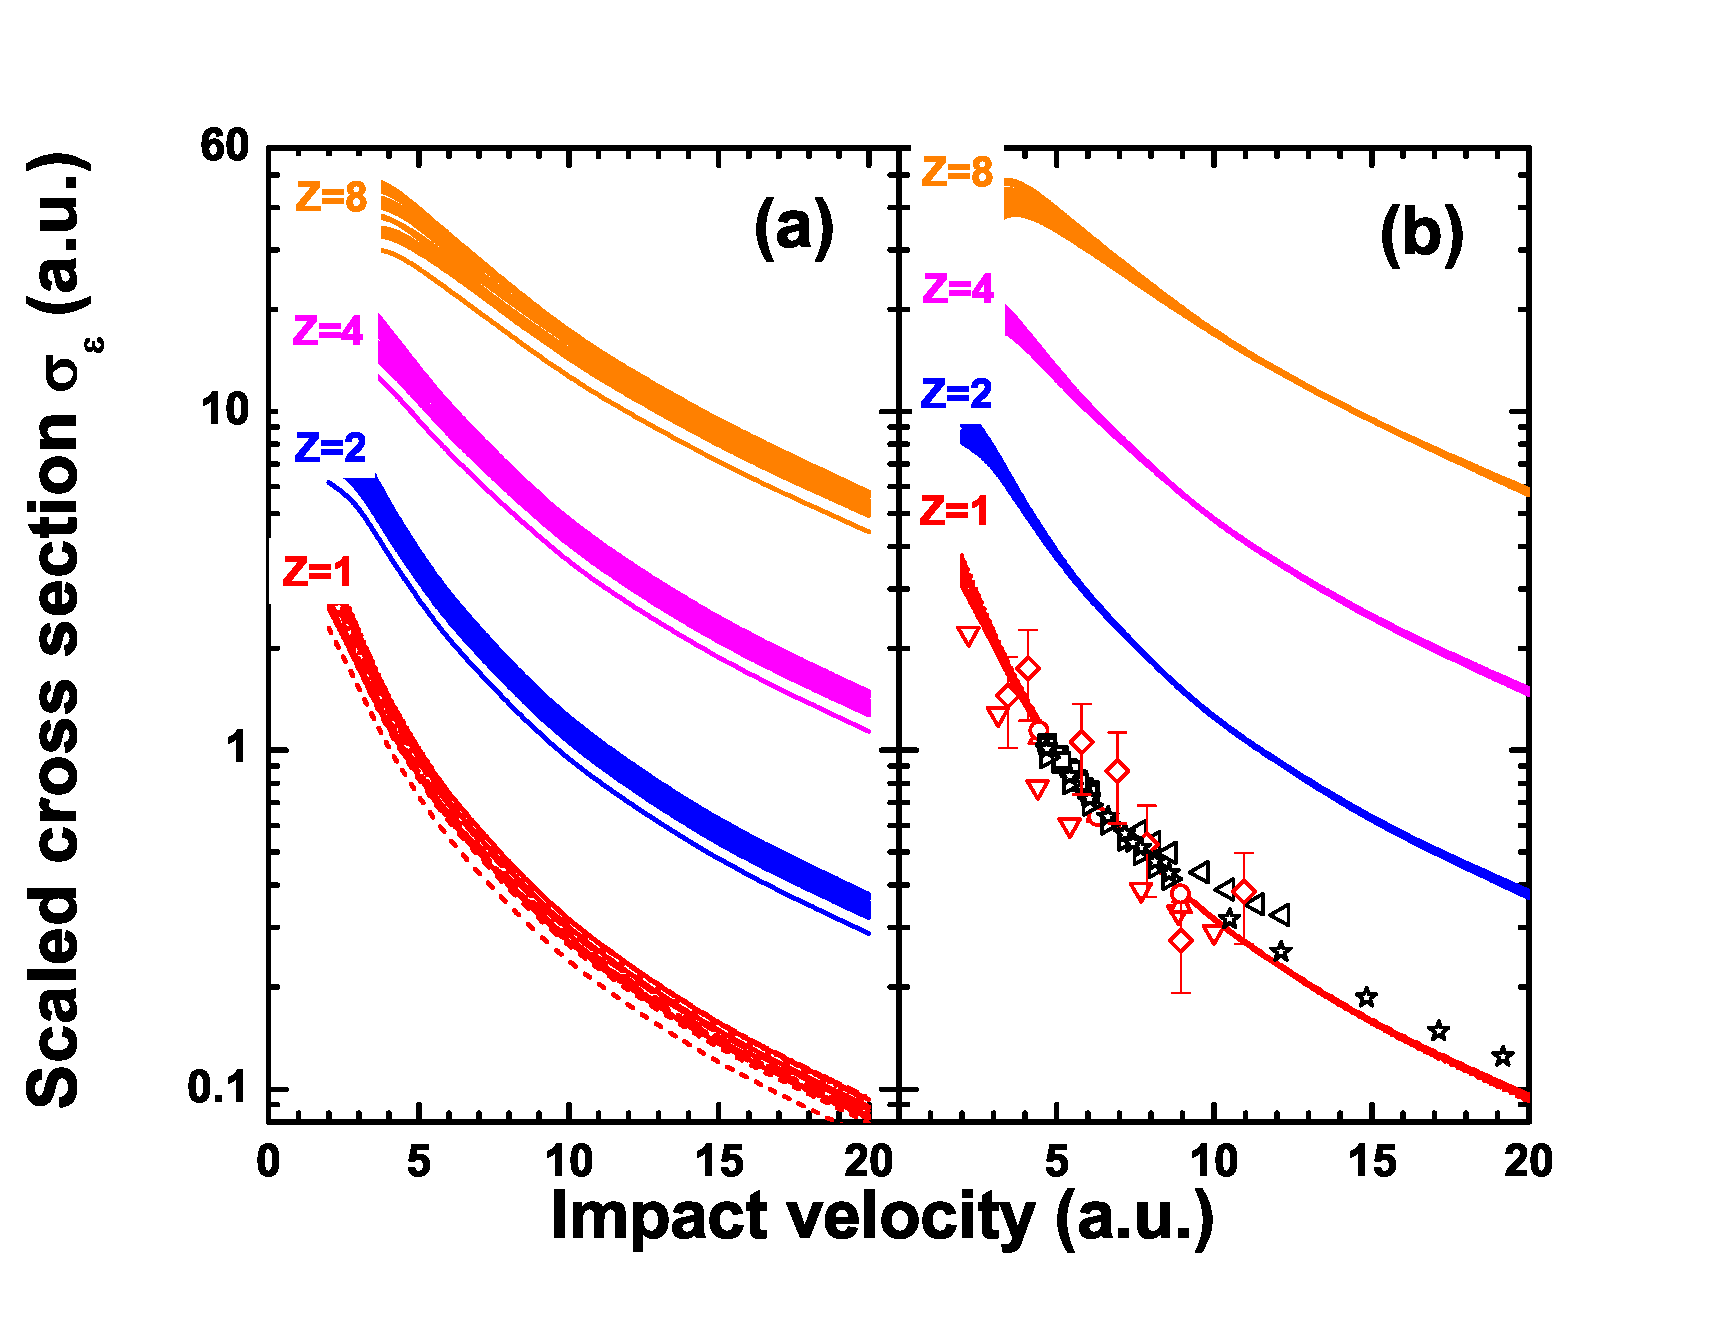
\includegraphics[width=0.75\textwidth]{figuras/Fig_finales/fig4.eps}
%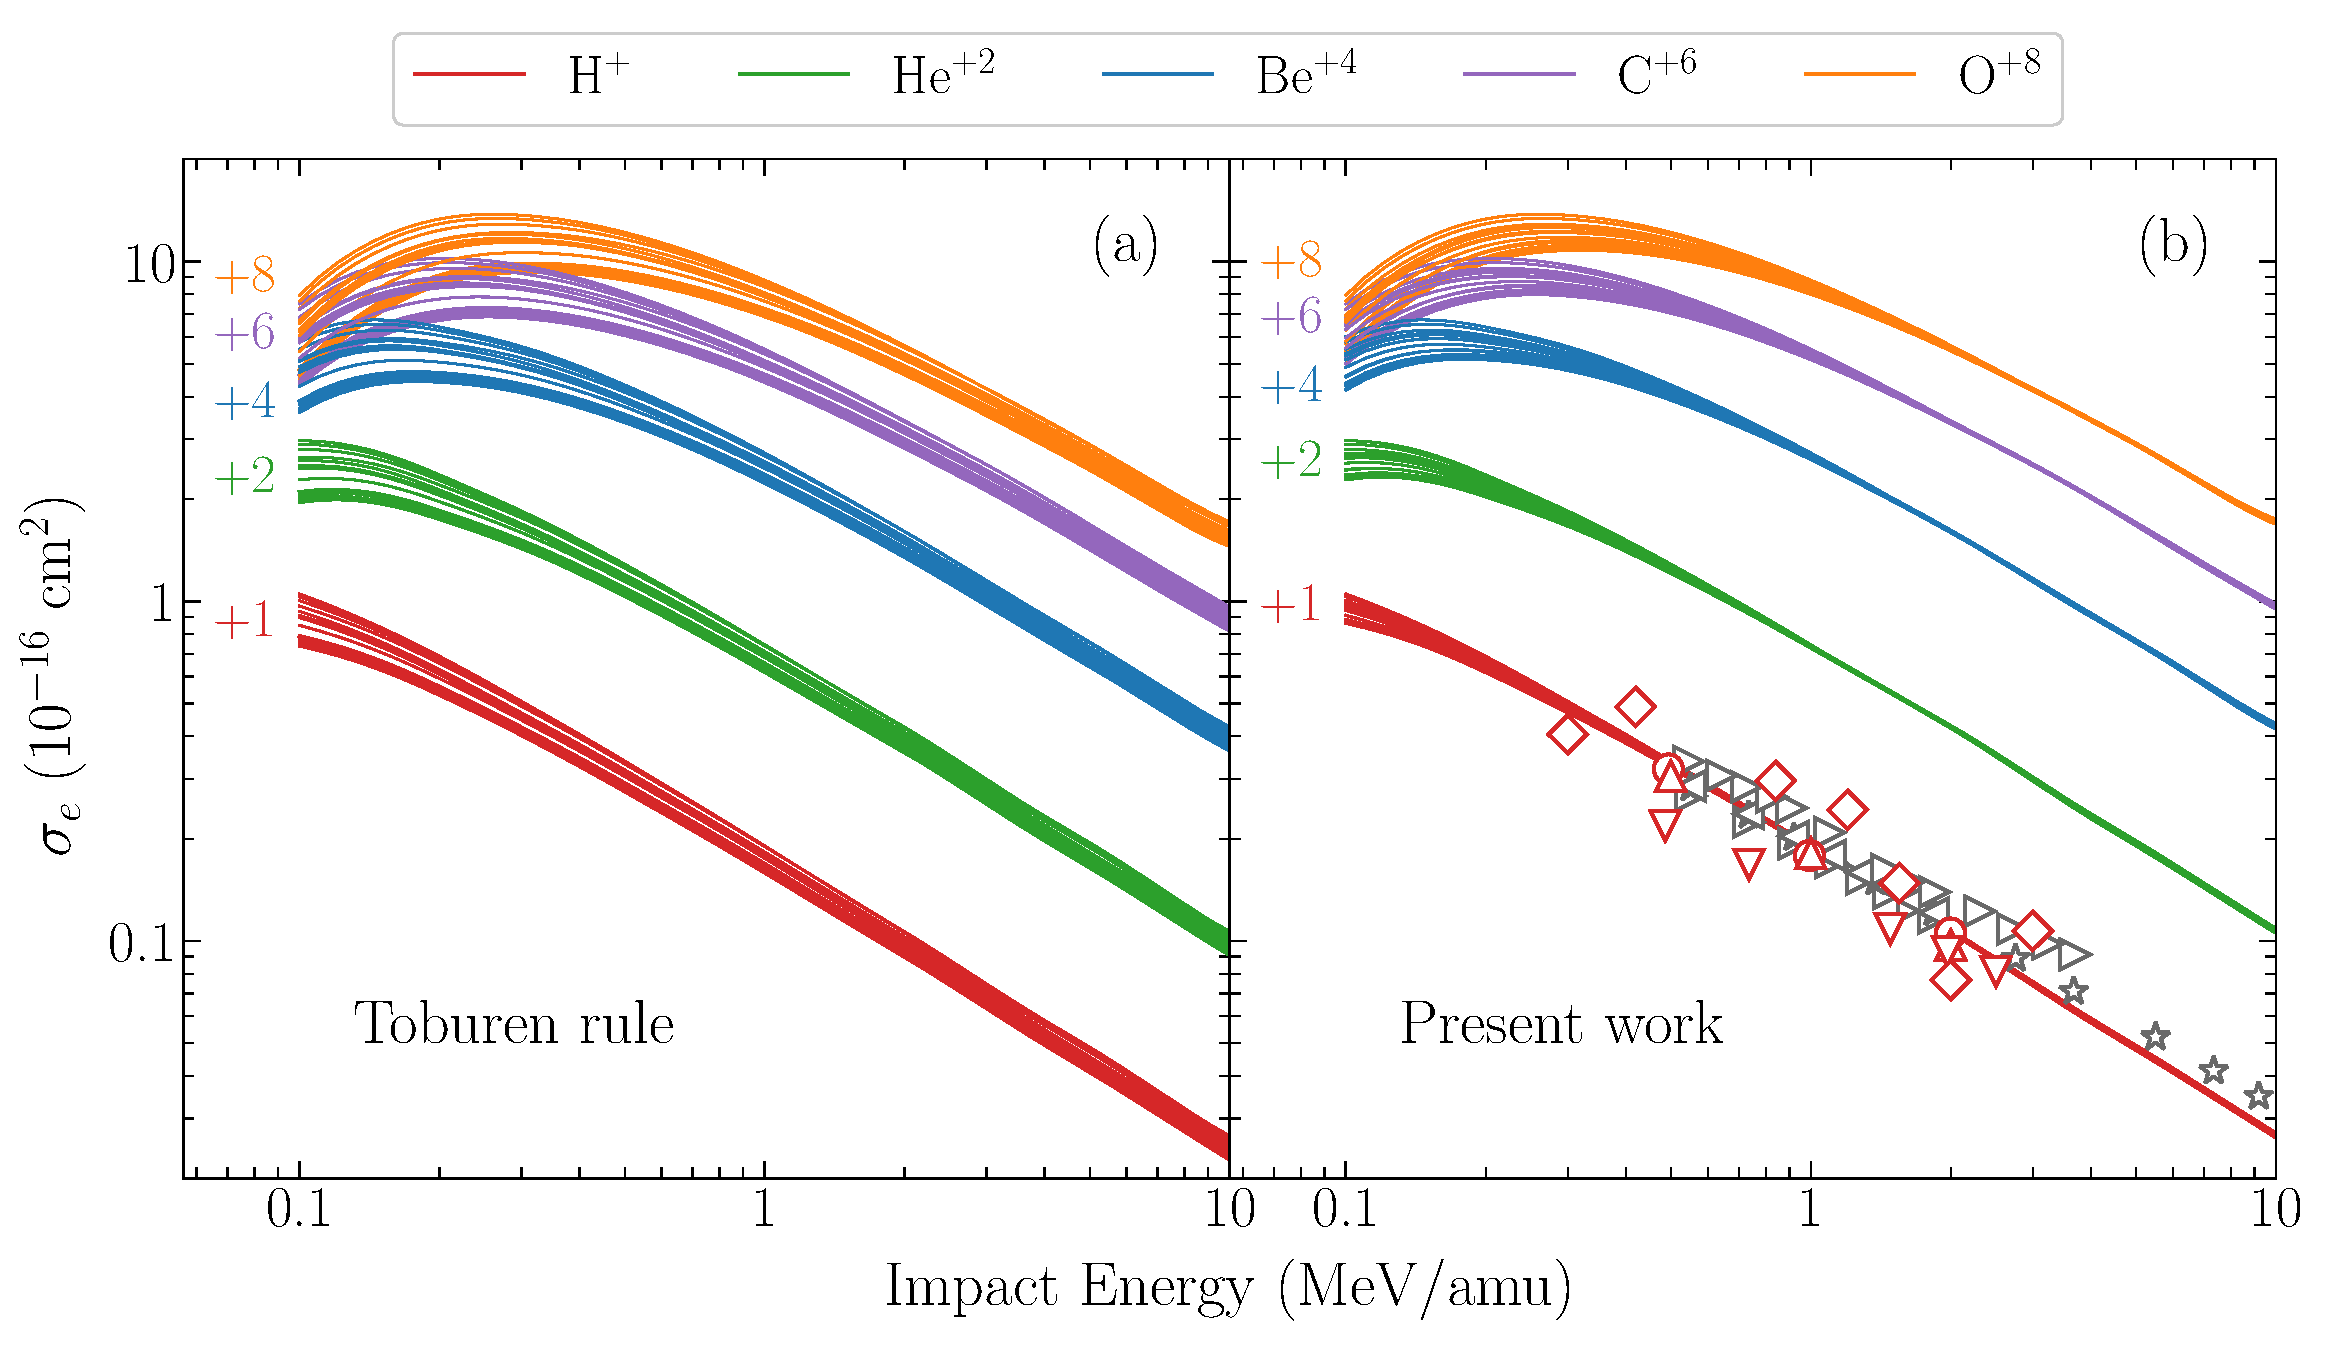
\includegraphics[width=0.9\textwidth]{figuras/molscaling85.eps}
\caption{Scaled ionization cross section per weakly bound electron using
(a)~the Toburen numbers $\nu_{\alpha}^T$, and (b) our proposed numbers
$\nu_{\alpha}^{\text{CDW}}$. Experiments: proton impact on 
\mbox{\Large$\circ$} adenine~\cite{iriki2011}, 
$\triangle$ uracil~\cite{itoh2013}, 
$\bigtriangledown$ pyrimidine~\cite{wolff2014} and $\meddiamond$ 
THF~\cite{wang2016}; electron impact on $\rhd$ pyrimidine~\cite{bug2017},
and $\lhd$, $\medstar$~\cite{wolf2019,fuss2009} THF.}
\label{fig:newscaling}
\end{figure*}

By implementing the SSM, we computed the scaled CDW cross sections 
$\sigma_{e}^T$ for the molecular targets of Table~\ref{tab:families}.
Our results are shown in Fig.~\ref{fig:newscaling}a as a function of 
the impact energy for different projectile charges. Although the 
Toburen scaling holds for high energies, its performance is still not 
satisfactory: the universal band is quite broad, as can be noted in 
Fig.~\ref{fig:newscaling}a.

%%%%%%%%%%%%%%%%%%%%%%%%%%%%%%%%%%%%%%%%%%%%%%%%%%%%%%%%%%%%%%%%%%%%%%%%
\subsubsection{New scaling}
%%%%%%%%%%%%%%%%%%%%%%%%%%%%%%%%%%%%%%%%%%%%%%%%%%%%%%%%%%%%%%%%%%%%%%%%

The departure of our theoretical 
results from the Toburen rule can be easily understood 
by inspecting Fig.~\ref{fig:atomscaling}. It can be noted that the 
rule $\sigma_{\alpha}/\nu_{\alpha}^T\sim \sigma_{e}^T$, approximatelly 
constant, is not well satisfied by the CDW. 
For example, Fig.~\ref{fig:atomscaling} shows that the cross sections
for O are actually very similar to the cross sections for C, suggesting 
4 active electrons in O instead of 6. In the same way, the number of
active electrons for N, P and S are also different from the 
$\nu_{\alpha}^T$ of Eq.~(\ref{eq:nelec}). 

Based on the CDW results, we propose a new scaling,
\begin{equation}
\sigma_{e}=\frac{\sigma_M}{n_e'},
\label{32} 
\end{equation}
where $n_e'=\sum_{\alpha}n_{\alpha}\nu_{\alpha}^{\text{CDW}}$, and 
$\nu_{\alpha}^{\text{CDW}}$ are the numbers of active electrons
per atom obtained from the CDW ionization cross sections for 
different ions in H, C, N, O, P , and S targets, given as follows,
\begin{equation}
\nu_{\alpha }^{\text{CDW}} \sim\left\{ 
\begin{array}{ll}
1, & \text{for H,} \\
4, & \text{for C, N, and O,} \\ 
4.5, & \text{for P and S}\,.
\end{array}
\right. 
\label{eq:scalingCDW}
\end{equation}

The new scaled cross sections $\sigma_{e}$ are plotted in 
Fig.~\ref{fig:newscaling}b. 
A much better sharp band is observed, especially for impact energies 
$E=(0.5-8)$~MeV/amu for $Z=1$ and $Z=2$, and $E=(2.5-8)$~MeV/amu for 
$Z>2$. In fact, the experimental data for ionization of 
adenine~\cite{iriki2011}, uracil~\cite{itoh2013}, 
pyrimidine~\cite{wolff2014} and THF~\cite{wang2016} by proton impact in
Fig.~\ref{fig:newscaling}b seems to corroborate the new scaling. 
We also included the electron impact ionization measurements with 
equivelocity conversion on pyrimidine~\cite{bug2017}, and 
THF~\cite{bug2017,wolf2019,fuss2009}. 
It will be interesting to cross--check for experiments with higher 
projectile charge states. 

\begin{table}[H]
\begin{center}
\begin{tabular}{|ll|ll|ll|}
\hline
 Molecule & $n_e$ &Molecule          & $n_e$ & Molecule             & $n_e$\\
\hline
 H$_2$    & 2  & C$_2$H$_7$N         & 19    & C$_4$H$_5$N$_3$O     & 37   \\
 H$_2$O   & 6  & C$_4$H$_8$O         & 28    & C$_5$H$_6$N$_2$O$_2$ & 42   \\
 NH$_3$   & 7  & C$_4$H$_4$N$_2$     & 28    & C$_5$H$_5$N$_5$      & 45   \\
 CH$_4$   & 8  & C$_6$H$_6$          & 30    & C$_5$H$_5$N$_5$O     & 49   \\
 CH$_5$N  & 13 & C$_4$H$_4$N$_2$O$_2$& 36    & C$_5$H$_{10}$O$_5$P  & 54.5 \\
 \hline
\end{tabular}
\caption{New scaling numbers for some molecular targets of biological 
interest.}
\label{nn}
\end{center}
\end{table}

\begin{figure*}[t!]
\centering
%\includegraphics[width=0.75\textwidth]{figuras/Fig_finales/fig_recta.eps}
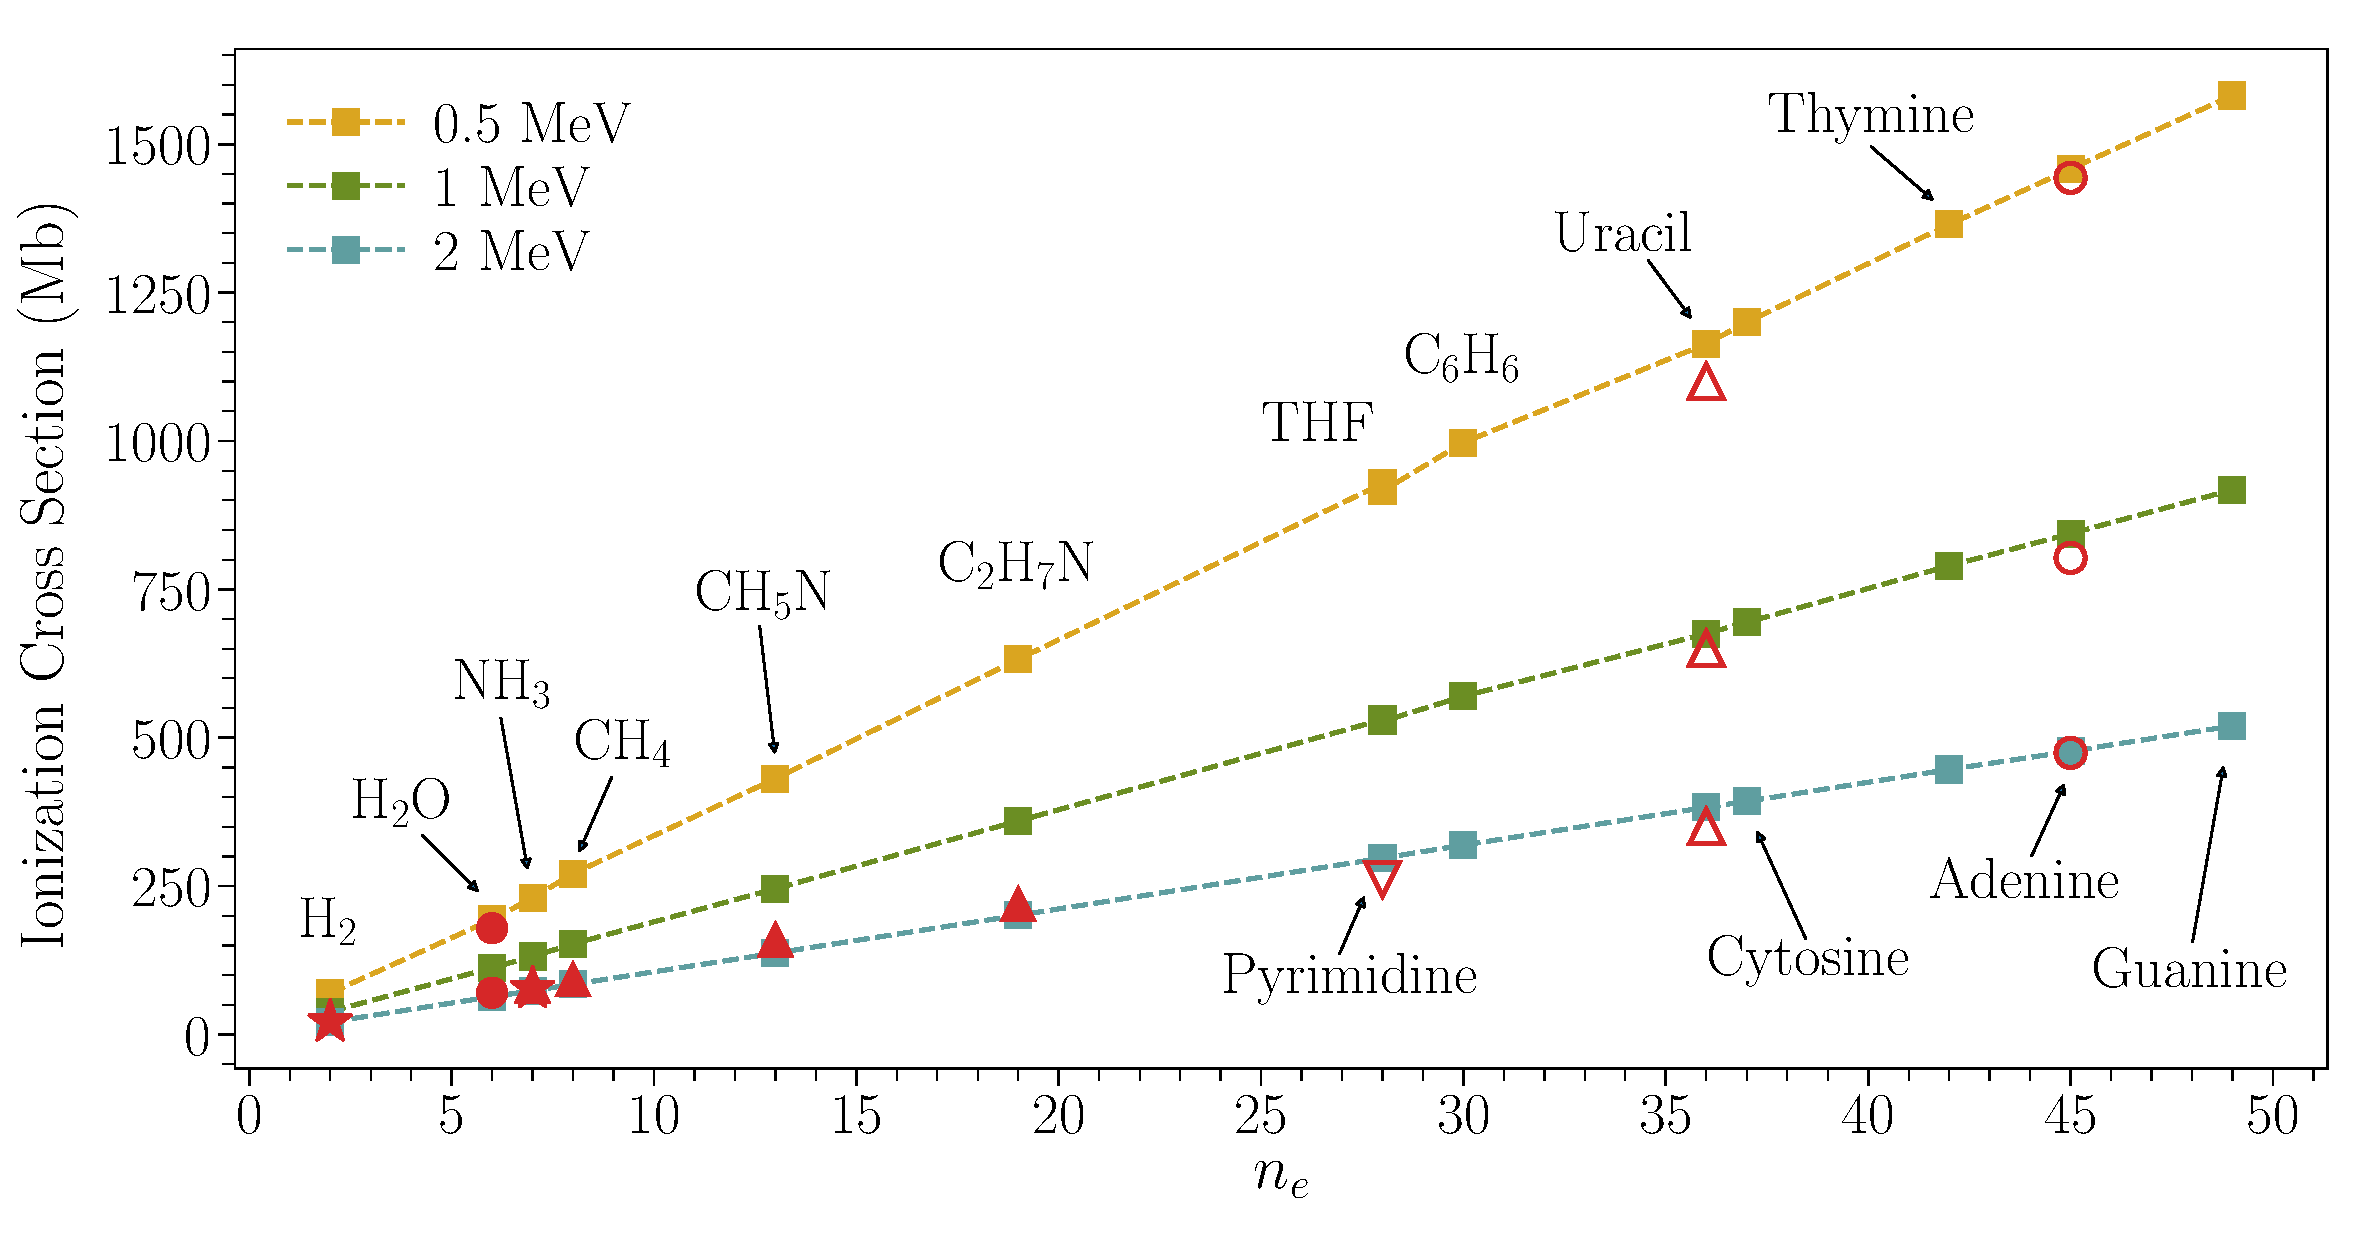
\includegraphics[width=0.75\textwidth]{figuras/scale_ne.eps}
\caption{Ionization cross sections by impact of protons at 0.5, 1 and 2 MeV
in terms of the number of active electrons given by Table~\ref{nn}.
Experiments: 
\mbox{\Large$\circ$}~adenine~\cite{iriki2011}, 
$\triangle$ uracil~\cite{itoh2013}, 
$\bigtriangledown$ pyrimidine~\cite{wolff2014}, 
$\blacktriangle$ C2H$_7$N, CH$_5$N, methane and amonia~\cite{lynch1976},
\mbox{\scriptsize$\bigstar$} amonia and H$_2$~\cite{rudd1985}, and 
\mbox{\Large$\bullet$} water~\cite{luna2007}.}
\label{fig:recta}
\end{figure*}

By using Eq.~(\ref{eq:scalingCDW}), we define new active electron 
numbers $n_e'$ for some molecular of interest in Table~\ref{nn}. 
These values are very different from the ones proposed by Toburen and 
used by other authors~\cite{itoh2013}.
Moreover, an alternative way of showing the scaling can be attained by 
plotting the ionization cross sections of molecules as a function of the 
number of active electrons from Table~\ref{nn}. Our findings are displayed 
in Fig.~\ref{fig:recta} for impact energies 0.5, 1 and 2 MeV. As can be 
noted, the computed CDW ionization cross sections for all the molecules  
show a linear dependence with the number of electrons from Table~\ref{nn}. 
We obtain similar results even for $E=10$~MeV. The comparison with the 
experimental data available shows very nice agreement, from the smallest 
molecules, H$_2$, H$_2$O and CH$_4$, up to the most complex ones, like 
adenine. For electron impact data, the experimental data was interpolated
between close neighboors.

Finishing the present work we noted an accepted manuscript by 
Luedde~{\it et al.} \cite{luedde2019} who also noted a similar scaling 
at least for C, N, and O and reinforces the present finding.

%%%%%%%%%%%%%%%%%%%%%%%%%%%%%%%%%%%%%%%%%%%%%%%%%%%%%%%%%%%%%%%%%%%%%%%%
\subsection{Molecular structure of targets}
%%%%%%%%%%%%%%%%%%%%%%%%%%%%%%%%%%%%%%%%%%%%%%%%%%%%%%%%%%%%%%%%%%%%%%%%

To test the range of validity of the SSM, we performed a full molecular 
structure calculation of five nucleobases. We employed the {\sc gamess} 
code and used the 6-31G(d,p) basis set, which includes polarization 
functions for all the atoms. The calculations were carried out 
implementing the B3LYP functional~\cite{Becke1993,Stephens1994} to 
account for the correlation and exchange effects. 

The molecular binding energies of the valence electrons for adenine, 
cytosine, guanine, thymine and uracil are shown in Fig.~\ref{fig:bindener}. 
We can compute the center of gravity of these molecular energy levels as 
an average weighted by the electronic occupation number. The results 
obtained from the full molecular calculation are given in the first row
of Table~\ref{tab:gravener}. Similarly, we can compute the baricenter
of the energy levels defined by the Toburen rule and the new rule, given by
Eq.~(\ref{eq:scalingCDW}), which are also given in 
Table~\ref{tab:gravener}. The average energy values obtained from the
Toburen rule are around 20\% of the full molecular ones. Surprisingly, 
the new scaling rule gives a significant 
improvement in the average energy values, reducing the relative errors
to about~7\%. This improvement would seem to indicate that the new 
scaling is appropiate.

\begin{figure*}[t!]
\centering
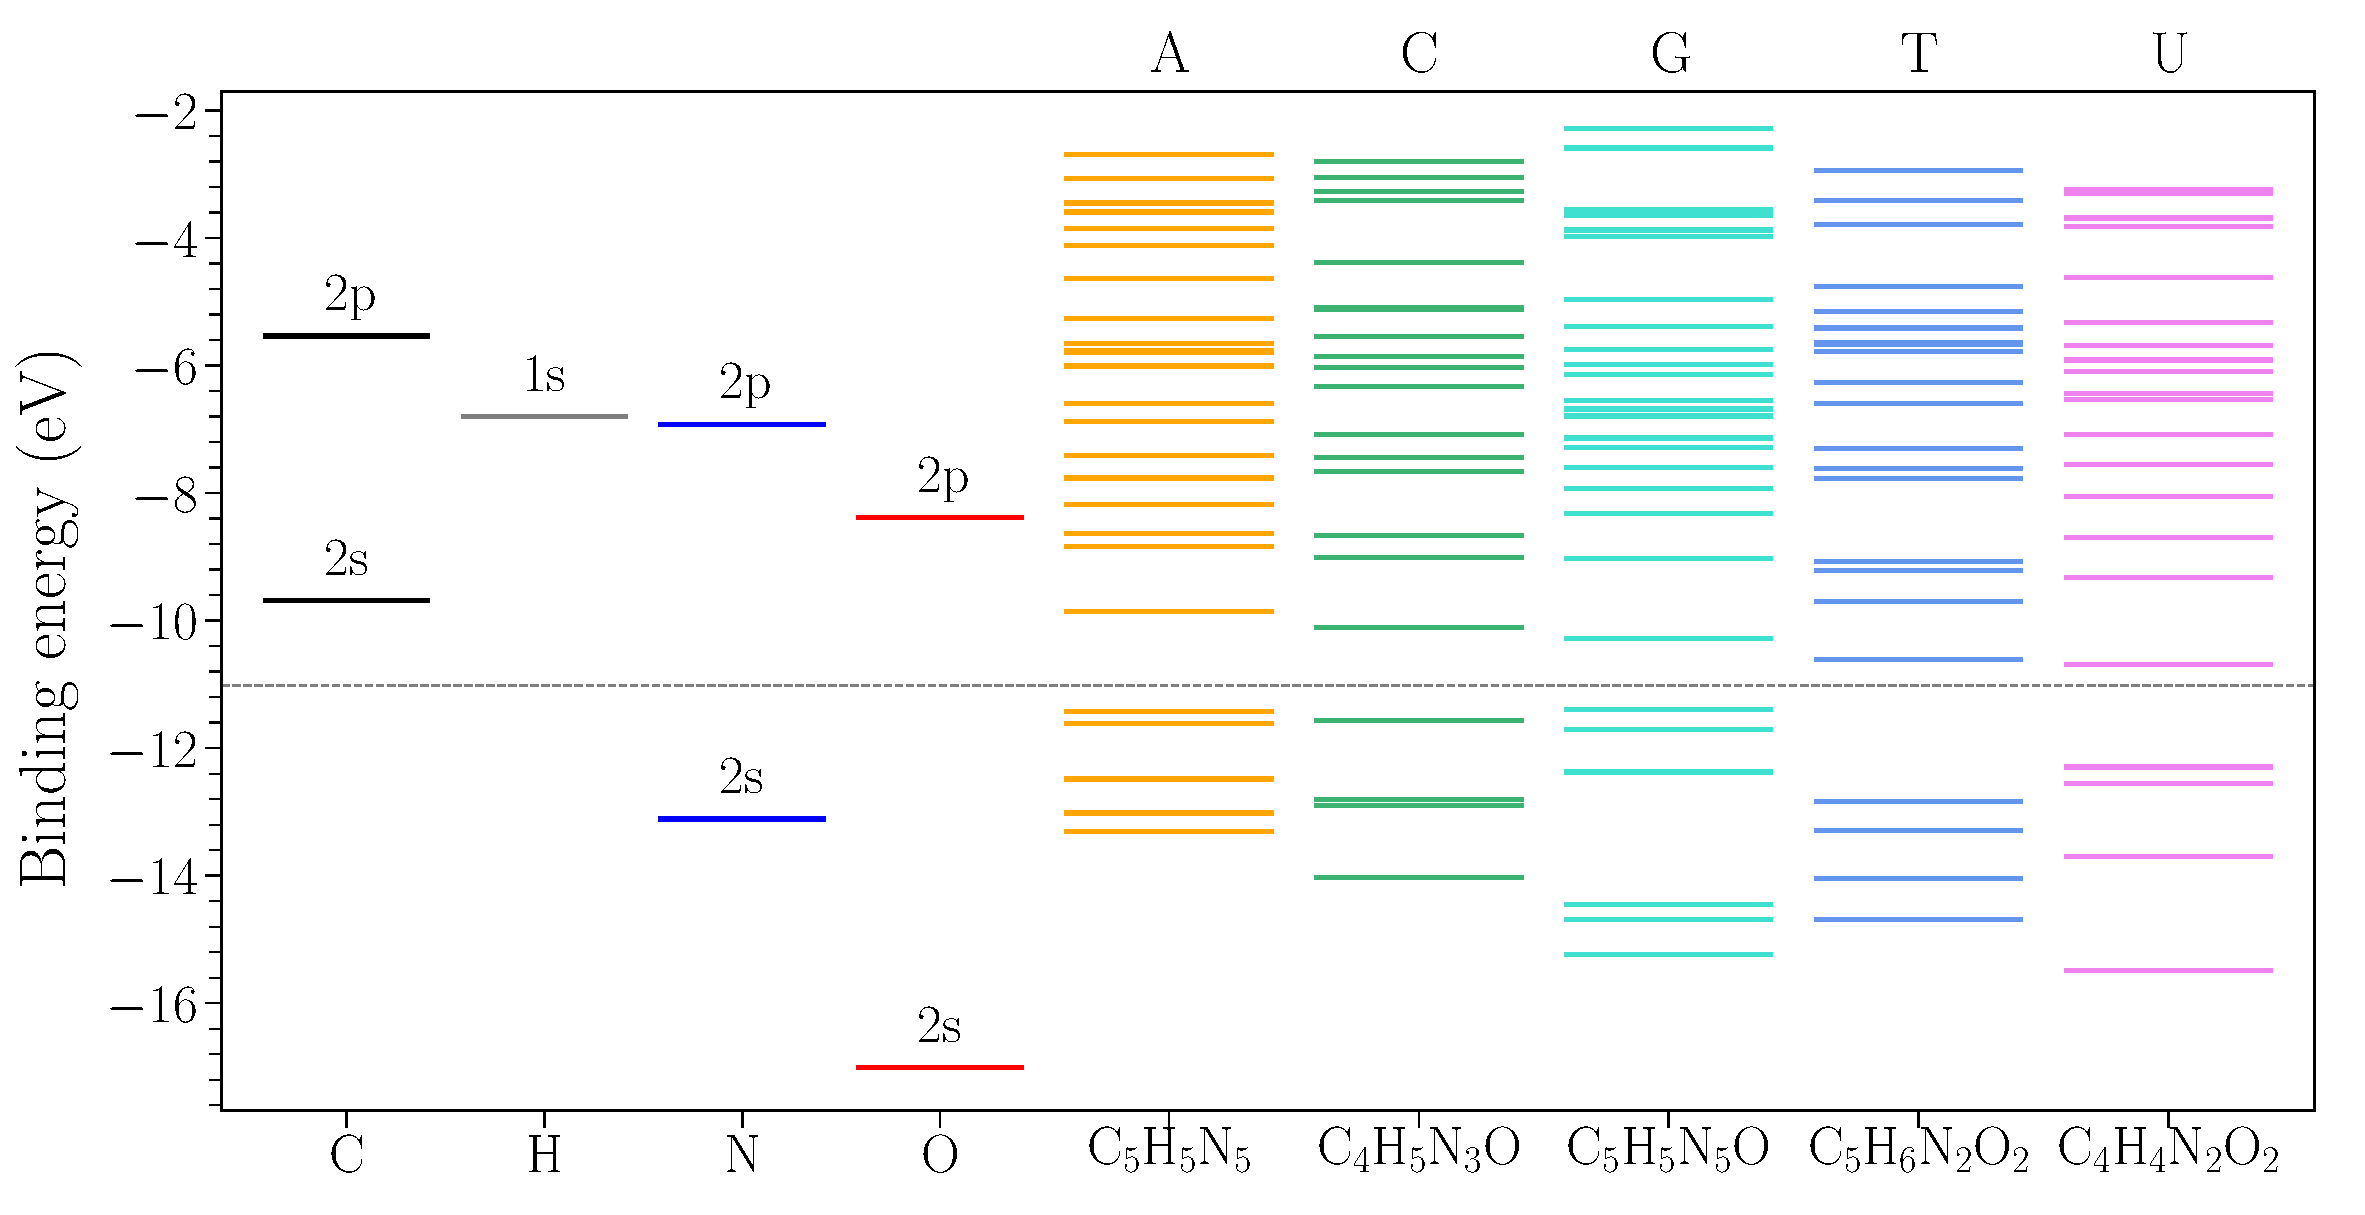
\includegraphics[width=0.9\textwidth]{figuras/levelsDNA.eps}
\caption{Theoretical molecular binding energies for adenine, cytosine, 
guanine, thymine and uracil compared to those of atomic constituents.}
\label{fig:bindener}
\end{figure*}

\begin{table}[H]
\begin{center}
\begin{tabular}{|c|ccccc|}
\hline
 \multirow{2}{*}{$E_{\text{av}}$ (eV)} & A & C & G & T & U \\
 & C$_5$H$_5$N$_5$ & C$_4$H$_5$N$_3$O & 
   C$_5$H$_5$N$_5$O & C$_5$H$_6$N$_2$O$_2$ & C$_4$H$_4$N$_2$O$_2$ \\
\hline
 Theoretical calc. & $-7.1955$ & $-6.9058$ & $-7.4725$ & $-7.5304$ & $-7.6224$ \\
 Toburen rule  & $-8.4236$ & $-8.6743$ & $-8.7275$ & $-8.7947$ & $-9.0022$ \\
 Present work & $-7.9027$ & $-7.8639$ & $-7.9420$ & $-7.8066$ & $-7.8839$ \\
%                 17%         25%         17%         17%         18%         
%                 10%         13%         6%          4%          3%
\hline
\end{tabular}
\caption{Center of gravity of the molecular energy levels of five 
nucleobases.}
\label{tab:gravener}
\end{center}
\end{table}


Furthermore, on the left side of the Fig.~\ref{fig:bindener}, we show 
the atomic Hartree--Fock energies of the constituent elements, which 
gives an insight on the distribution of the weakly bound electrons. 
A dashed line around $-11$~eV is drawn to separate the band in two. 
We can consider the atomic energy levels above this line as the ones
corresponding to the weakly bound electrons from Eq.~(\ref{eq:scalingCDW}).
For example, the $2s$ and $2p$ electrons of carbon are placed above
the separating line, which corresponds to the 4 electrons given by 
Eq.~(\ref{eq:scalingCDW}). In the case of O, only the 4 electrons of 
the $2p$ orbitals are located above the separating line, which 
corresponds to the number of weakly bound electron given by 
our new scaling. 
The N case is not as straightfoward; the $\nu_{\alpha }^{\text{CDW}}$ 
value given for N would suggest that some $2s$ electrons corresponding 
to the molecular squeme are also weakly bonded, leading to 4 electrons.



\subsubsection{A modified stoichiometric model}

The SSM considers the molecule to be assembled by isolated neutral atoms, 
which is definitively unrealistic. A first improvement can be suggested 
by assuming that the atoms are not neutral and that they have an uneven
distribution of electrons within the molecule; this distribution can be
given by an effective charge $q_{\alpha}$. A possible value for 
$q_{\alpha}$ is given by the Mulliken charge. However, there are a wide
variety of charge distributions, such as the net or natural atomic
charge~\cite{lee2003}, the L\"owdin charge, etc.

Consider that the total amount of electrons $Q_{\alpha }$ on the element
$\alpha$ are equally distributed on all the $\alpha$ atoms. Therefore, 
each element $\alpha$ will have an additional charge: 
$q_{\alpha}=Q_{\alpha}/n_{\alpha}$, which can be positive or negative.
This value will depend on the relative electronegativity value with 
respect to the other atoms~\cite{rappe1991}. Now, instead of an
integer number of elements $n_{\alpha}$ of the atom $\alpha$, we have a 
fractional number of atoms given by 
\begin{equation}
n_{\alpha }^{\prime }=n_{\alpha }-
\frac{q_{\alpha }}{\nu_{\alpha }^{\text{CDW}}}
\label{eq:newstoi}
\end{equation}%
In the case of neutral atoms, $q_{\alpha}=0$ and we recover 
$n_{\alpha}^{\prime}=n_{\alpha}$, as it should be. 
In Table~\ref{tab:newstoi}, we display the average effective charge 
per atom $q_{\alpha}$ of C, H, N and O, for five DNA molecules. 
The charges were obtained from the full molecular calculation described 
above.

\begin{table}[H]
\begin{center}
\begin{tabular}{|p{0.12\textwidth}|p{0.07\textwidth}|p{0.07\textwidth}|p{
0.07\textwidth}|p{0.07\textwidth}|p{0.25\textwidth}|}
\hline
Element & C & H & N & O & New stoichiometry \\
\hline
Adenine & +0.32 & +0.23 & --0.55 &       & 
C$_{4.92}$H$_{4.77}$N$_{5.14}$ \\ 
\hline
Cytosine & +0.28 & +0.21 & --0.56 & --0.53 & 
C$_{3.93}$H$_{2.79}$N$_{5.14}$O$_{1.13}$ \\ 
\hline
Guanine & +0.46 & +0.20 & --0.58 & --0.36 & 
C$_{4.89}$H$_{4.80}$N$_{5.15}$O$_{1.09}$ \\ 
\hline
Thymine & +0.20 & +0.19 & --0.54 & --0.52 & 
C$_{4.95}$H$_{1.81}$N$_{6.13}$O$_{2.13}$ \\ 
\hline
Uracil & +0.31 & +0.22 & --0.59 & --0.47 & 
C$_{3.92}$H$_{1.78}$N$_{4.15}$O$_{2.12}$ \\ 
\hline
\end{tabular}
\caption{Average effective Mulliken charge per atom $q_{\alpha}$, and 
new stoichiometric formula defined by Eq.~(\ref{eq:newstoi}) for five 
DNA molecules.}
\label{tab:newstoi}
\end{center}
\end{table}


By implementing Eq.~(\ref{eq:newstoi}), it is possible to determine a 
new stoichiometric formula (last column of Table~\ref{tab:newstoi}). 
Now, instead of having an integer number of atoms $n_{\alpha}$, we obtain 
a fractional number $n_{\alpha}^{\prime}$. New molecular cross sections 
$\sigma^{\prime}_{M}=\sum_{\alpha}n_{\alpha}'\sigma_{\alpha}$ can be 
computed considering 
such values. Relative errors for the ionization cross sections were 
computed for the DNA bases from Table~\ref{tab:newstoi}. The differences 
obtained were less than 3\%, which indicates that the modified 
SSM is a quite robust model to handle these type of molecules within 
the range error expected for this model.

%%%%%%%%%%%%%%%%%%%%%%%%%%%%%%%%%%%%%%%%%%%%%%%%%%%%%%%%%%%%%%%%%%%%%%%%
\section{Conclusions}
%%%%%%%%%%%%%%%%%%%%%%%%%%%%%%%%%%%%%%%%%%%%%%%%%%%%%%%%%%%%%%%%%%%%%%%%

In this work we have encouraged the calculation of ionization cross 
sections of seventeen biological molecules containing H, C, N, O, P and 
S by impact of antiprotons, H$^{+}$, He$^{2+}$, Be$^{4+}$, C$^{6+}$, 
and O$^{8+}$. 
To that end we have employed the full CDW method including... and a 
simple stoichiometric model. 
The mean energy and angle of the emitted electrons, of importance in 
post-collisional radiation damage,  has also been calculated, showing 
a clear dependence with the ion charge $Z$. For a given target as $Z$ 
increases, $\overline{E}_{\alpha}$
increases, but $\overline{\theta}_{\alpha}$ decreases. At impact
energies larger than 1 MeV/amu, these values converge to the Born
approximation, which embodies the simple $Z^{2}$ law. 

Total ionization cross sections for adenine, cytocine, thymine, gaunine, 
uracil, DNA backbone, pyrimidine and THF are presented and compared 
with the the scarse available experiments. We explore the rule of 
Toburen which scales
all the molecular ionization cross section normalizing with certain 
number of
weakly bound or valence electrons. We found that ionization cross 
sections scales much better when normalizing with the number of active 
electrons in the collision obtained from the CDW results for atoms. 
This new scaling was tested with very good results for the six 
projectiles and seventeen molecules studied here. The comparison with 
the experimental data reinforce this results. Moreover, we also test 
the scaling by including experimental data of ionization of H$_2$, 
water, methane and ammonia by proton impact showing good agreement at
intermediate to high energies.
Finally, we performed full molecular calculations for the DNA basis. 
By inspecting the molecular binding energy from quantum mechanical
structure calculations, we were able to understand the number of 
electrons proposed in our new CDW-based scaling. We attempt to improve 
the stoichiometric model by using the Mulliken charge to get fractional
rather than integer proportions. It is interesting to remark that no 
substantial
correction was found, which indicates that the SSM works quite well.

The main objective of this article was to provide the tools to estimate 
any inelastic parameter parameter --such as emission angle, emitted mean
energy and cross section-- by the impact of any multicharged projectiles 
on any molecule containing H, C, N, O, P and S, with the help of the
stoichimetrical model. Our goal was quite ambitious, considering the
simplicity of our proposal. However, the present results show the 
validity of the simple stoichiometric model to estimate the ionization 
magnitude with an acceptable level of uncertainty.  

\bigskip

\begin{thebibliography}{99}


\bibitem{toburen1975} 
W. E. Wilson and L. H. Toburen. Electron emission from
proton --hydrocarbon-molecule collisions at 0.3--2.0 MeV. 
Phys. Rev. A 11, 1303 (1975).

\bibitem{toburen1976} 
D. J. Lynch, L. H. Toburen, and W. E. Wilson. Electron
emission from methane, ammonia, monomethylamine, and dimethylamine by 0.25
to 2.0 MeV protons. 
J. Chem. Phys. 64, 2616 (1976).


\bibitem{gamess}
M. W. Schmidt, K. K. Baldridge, J. A. Boatz, S. T. Elbert, M. S. Gordon, 
J. H. Jensen, S. Koseki, N. Matsunaga, K. A. Nguyen, S. J. Su, T. L. Windus, 
M. Dupuis, J. A. Montgomery 
J. Comput. Chem. 14, 1347-1363 (1993)

\bibitem{miraglia2008} 
J. E. Miraglia and M. S. Gravielle. Ionization of the
He, Ne, Ar, Kr, and Xe isoelectronic series by proton impact. 
Phys Rev A \textbf{78}, 052705 (2008)

\bibitem{miraglia2009} 
J. E. Miraglia, Ionization of He, Ne, Ar, Kr, and Xe
by proton impact: Single differential distributions. 
Phys. Rev. A \textbf{79}, 022708 (2009).

\bibitem{fainstein1988}
Fainstein P.D., Ponce V. H. and Rivarola R. D. 
J. Phys. B: At. Mol. Opt. Phys. \textbf{21} 287 (1988).

\bibitem{salvat1995}
Salvat, F., Fernández-Varea, J.M., Williamson, W.
Comput. Phys. Commun. \textbf{90}, 151--168 (1995)

\bibitem{mendez2016} 
A.M.P. Mendez, D.M. Mitnik, and J.E. Miraglia.
Depurated inversion method for orbital-specific exchange potentials. 
Int. J. Quantum Chem. 24 ,116 (2016).

\bibitem{mendez2018} 
A.M.P. Mendez, D.M. Mitnik, and J.E. Miraglia. Local Effective 
Hartree--Fock Potentials Obtained by the Depurated Inversion Method,
76. (2018).

\bibitem{montanari2017} 
Ionization probabilities of Ne, Ar, Kr, and Xe by
proton impact for different initial states and impact energies. 
Nucl. Instr. Meth. Phys. Res. B 407 (2017) 236-243.

\bibitem{miraglia2019} 
J. E. Miraglia. Shell-to-shell ionization cross
sections of antiprotons, H$^{+}$, He$^{+2},$ Be$^{+4},$ C$^{+6}$ and 
O$^{+8}$ on H, C, N, O, P, and S atoms To be published Archive 2019.


\bibitem{surdutovic2018} 
Multiscale approach to the physics of radiation
damage with ions. E. Surdutovich and A. V. Solov'yov, 
arXiv:1312.0897v, (2013)

\bibitem{abril2015} 
P. de Vera1, I. Abril, R. Garcia-Molina and
A.V.Solov'yov,\ Ionization of biomolecular targets by ion impact: input data
for radiobiological applications. 
Journal of Physics: Conference Series 438
(2013) 012015

\bibitem{Rudd1992} 
M. E. Rudd, Y.-K. Kim,, D. H. Madison and T. J. Gay.
Electron production in proton collisions with atoms and molecules: energy
distributions. 
Rev. Mod. Phys. \textbf{64}, 44-490 (1992).



\bibitem{iriki2011}
Y. Iriki, Y. Kikuchi, M. Imai, and A. Itoh
Phys. Rev. A \textbf{84} 052719 (2011).

\bibitem{rahman2016}
M. A. Rahman and E. Krishnakumar,
Electron ionization of DNA bases,
J. Chem. Phys. \textbf{144}, 161102 (2016).

\bibitem{mozejko2003}
P. Mozejko and L. Sanche, 
Cross section calculations for electron scattering from DNA and RNA bases.
Radiat Environ. Biophys \textbf{42}, 201 (2003).

\bibitem{tan2018}
H. Q. Tan, Z. Mi, and A. A. Bettiol, 
Simple and universal model for electron-impact ionization of complex 
biomolecules, 
Phys. Rev. E \text{97}, 032403 (2018)

\bibitem{itoh2013} 
A. Itoh, Y. Iriki, M. Imai, C. Champion, and R. D. Rivarola, 
Cross sections for ionization of uracil by MeV-energy-proton impact, 
Phys. Rev. A \textbf{88}, 052711 (2013).

%\bibitem{} in energy and angles~,

\bibitem{agnihotri2012}
A. N. Agnihotri, S. Kasthurirangan, S. Nandi, A.
Kumar, M. E. Galassi, R. D. Rivarola, O. Foj\'{o}n, C. Champion, J. Hanssen,
H. Lekadir, P. F. Weck, and L. C. Tribedi. 
Ionization of uracil in collisions with highly charged carbon and oxygen 
ions of energy 100 keV to 78 MeV. 
Phys. Rev. A \text{85}, 032711 (2012).

\bibitem{agnihotri2013}
A N Agnihotri, S Kasthurirangan, S Nandi, A Kumar, C Champion,, H Lekadir, 
J Hanssen, P FWeck, M E Galassi, R D Rivarola, O Fojon and L C Tribedi, 
Absolute total ionization cross sections of uracil (C$_4$H$_4$N$_2$O$_2$) in 
collisions with MeV energy highly charged carbon, oxygen and fluorine ions
J. Phys. B \textbf{46}, 185201 (2013).

\bibitem{champion2012} 
C Champion, M E Galassi, O Foj\'{o}n, H Lekadir, J Hanssen, R D Rivarola,
P F Weck, A N Agnihotri, S Nandi, and L C Tribedi. 
Ionization of RNA-uracil by highly charged carbon ions.
J. Phys.: Conf. Ser. \textbf{373}, 012004 (2012).

\bibitem{wolff2014}
W. Wolff, H. Luna, L. Sigaud, A. C. Tavares, and E. C. Montenegro
Absolute total and partial dissociative cross sections of pyrimidine
at electron and proton intermediate impact velocities
J. Chem. Phys. \textbf{140}, 064309 (2014).

\bibitem{bug2017}
M. U. Bug, W. Y. Baek, H. Rabus, C. Villagrasa, S. Meylan, A. B. Rosenfeld,
An electron-impact cross section data set (10 eV--1 keV) of DNA
constituents based on consistent experimental data: A requisite for 
Monte Carlo simulations,
Rad. Phys. Chem. \textbf{130} 459--479 (2017).

\bibitem{wang2016}
M. Wang, B. Rudek, D. Bennett, P. de Vera, M. Bug, T. Buhr, W. Y. Baek, 
G. Hilgers, H. Rabus, 
Cross sections for ionization of tetrahydrofuran by protons at energies 
between 300 and 3000 keV
Phys. Rev. A \textbf{93}, 052711 (2016).

\bibitem{wolf2019}
W. Wolff, B. Rudek, L. A. da Silva, G. Hilgers, E. C. Montenegro, 
M. G. P. Homem,
Absolute ionization and dissociation cross sections of tetrahydrofuran:
Fragmentation--ion production mechanisms
J. Chem. Phys. \textbf{151}, 064304 (2019).

\bibitem{fuss2009}
M. Fuss, A. Muñoz, J. C. Oller, F. Blanco, D. Almeida, P. Limão-Vieira, 
T. P. D. Do, M. J. Brunger, G. García,
Electron-scattering cross sections for collisions with tetrahydrofuran 
from 50 to 5000 eV
Phys. Rev. A \textbf{80}, 052709 (2009).

\bibitem{lynch1976}
D. J. Lynch, L. H. Toburen, and W. E. Wilson,
Electron emission from methane, ammonia, monomethylamine, and
dimethylamine by 0.25 to 2.0 MeV protons
J. Chem. Phys. \textbf{64}, 2616 (1976).

\bibitem{rudd1985}
M.E. Rudd, Y.-K. Kim, D.H. Madison, J.W. Gallagher,
Electron production in proton collisions: total cross sections,
Review of Modern Physics, \textbf{57}, 965--994 (1985).

\bibitem{luna2007}
H. Luna, A. L. F. de Barros, J. A. Wyer, S. W. J. Scully, J. Lecointre, 
P. M. Y. Garcia, G. M. Sigaud, A. C. F. Santos, V. Senthil, M. B. Shah, 
C. J. Latimer, and E. C. Montenegro,
Water-molecule dissociation by proton and hydrogen impact,
Phys. Rev. A \textbf{75} 042711 (2007).

\bibitem{luedde2019}
H J Luedde et al 2019 
J. Phys. B: At. Mol. Opt. Phys. in press https://doi.org/10.1088/1361-6455/ab3a63

\bibitem{Becke1993}
A. D. Becke, 
J. Chem. Phys. 98, 5648-5652 (1993) 

\bibitem{Stephens1994}
P. J. Stephens, F. J. Devlin, C. F. Chabalowski, M. J. Frisch,
J. Phys. Chem. 98, 11623-11627 (1994) 

\bibitem{lee2003} 
Jung-Goo Lee, Ho Young Jeong, and Hosull Lee, Charges of
Large Molecules Using Reassociation of Fragments. 
Bull. Korean Chem. Soc.24 2003, 369 .

\bibitem{rappe1991} 
A. K. Rappe, A. K.and W. A. Goddard III,. 
J. Phys. Chem. \textbf{95 (}1991) 3358.

%\bibitem{pimblott2007} 
%S.M. Pimblott and J. A. LaVerne, Radiation
%Physics and Chemistry 76, 1244-1247 (2007)


%\bibitem{clementi}
%E. Clementi, C. Roetti,
%At. Data Nucl. Data Tables 14, 177--478 (1974).




\end{thebibliography}

\end{document}
